\section{Charged leptons in cosmic plasma}\label{Electron}

Charged leptons played significant roles in the dynamics and evolution of the early Universe. They were kept in equilibrium via electromagnetic and weak interactions.  In this chapter, I examine a dynamical model of the abundance of charged leptons $\mu^\pm$ and $e^\pm$ in the early Universe obtaining their disappearance temperature, the condition when they disappear from the particle inventory. Of particular interest is the dense electron-positron plasma present during the early Universe evolution. I study the damping rate and the magnetization process in this dense $e^\pm$ plasma in the early Universe.


%{Introduction\daggerfootnote{This chapter has been published previously as \citet{Gottbrath1999}.}}
%~~~~~~~~~~~~~~~~~~~~~~~~~~~~~~~~~~~~~~~~~~~~~~~~~

\section{Overview of charge leptons in early Universe}
%In this section we will focus on the following:
%\begin{itemize}
%    \item Charged leptons in early universe
%    \item Remarks on tau leptons
%\end{itemize}


%In the early universe, charged leptons are kept equilibrium with the cosmic plasma via electromagnetic and weak interactions which played significant roles in the dynamics and evolution of the Universe.  For example, the present $e^\pm$ in early universe can affect  the neutrino decoupling, photon heating, and big bang nucleosynthesis. Although, the massive lepton $\tau^\pm, \mu^\pm$ decay into light leptons ($\nu$, $l^\pm$) and hadrons in their lifespan. These high-energy leptons ($\nu$, $l^\pm$) originating from the decay of $\tau^\pm, \mu^\pm$ continue played a significant role in shaping the particle energy distribution which can affect the property of cosmic plasma.



The $\tau^\pm$ leptons can undergo various decay processes via the weak interaction in the early Universe, and is the only charged lepton that can decay into hadrons because of its heavy mass ($m_\tau=1776.86$ MeV). The principle decay channels of $\tau^\pm$ are given by
\begin{align}
&\tau^-\rightarrow\nu_\tau+e^-+\bar{\nu}_e,\qquad \tau^-\rightarrow\nu_\tau+\mu^-+\bar{\nu}_\mu,\\
&\tau^-\rightarrow\nu_\tau+\pi^-,\qquad\qquad\,\tau^+\rightarrow\bar{\nu}_\tau+\pi^+,
\end{align}
 where the vacuum lifespan for $\tau^\pm$ is given by ~[\cite{ParticleDataGroup:2022pth}]
\begin{align}
&\tau_{\tau}=(290.3\pm0.5)\times10^{-15}\,\mathrm{sec}.
\end{align}

Moreover, following the decay of $\tau^\pm$ into pions, these pions subsequently decay into a muon and a neutrino through the reaction
\begin{align}
\pi^-\rightarrow\nu_\mu+\mu^-,\qquad\qquad\,\pi^+\rightarrow\bar{\nu}_\mu+\mu^+,
\end{align}
with pion vacuum lifespan $\tau_\pi=2.6033\times10^{-8}$ sec~[\cite{ParticleDataGroup:2022pth}].
In this scenario, $\tau^\pm$ disappears from the Universe via multiparticle decay processes.
These decay processes can contribute as one of the sources for the production of neutrinos and muons in the early Universe.

The $\mu^\pm$ lepton abundance is an important quantity required for the understanding of several fundamental questions regarding properties of the primordial Universe,  particularly in relation to the freeze-out of strangeness flavor in the early Universe. We recall that the strangeness decay often proceeds into muons, energy thresholds permitting, as the charged kaons K$^\pm$ have a 63\% branching into $\mu+\bar \nu_\mu$. Should muons fall out of thermal abundance equilibrium this would directly impact the detailed balance back-reaction processes. Another, indirect influence on strangeness in early Universe arises through the nearly exclusive decay of charged pions into $\mu+\bar \nu_\mu$. Without chemical abundance equilibrium this back reaction stops too impacting pions and thus all other hadronic particles in the Universe. 

On the other hand, we will show that the lightest charged leptons $e^\pm$ can persist via the reaction $\gamma\gamma\to e^-e^+$ until the temperature $T=20$ keV in the early Universe.  After $T=20$ keV, the positron rapidly disappears through annihilation, leaving only residual electrons to maintain the Universe's charge neutrality. The existence of an electron-positron plasma plays a pivotal role in several aspects of the early Universe as follows: 

1. The role of electron-positron plasma has not received the appropriate attention in the days of precision Big-Bang nucleosynthesis studies. The standard BBN model indicates that the synthesis of light elements typically takes place at temperatures around  $86\,\mathrm{keV}>T_{BBN}>50\,\mathrm{keV}$~[\cite{Pitrou:2018cgg}]. Within this temperature range there are millions of electron-positron pairs per charged nucleon, providing an electron-positron-rich plasma environment for nucleosynthesis which leads to modifications in the Coulomb potential due to the screening effect. Furthermore, the electron-positron densities can reach millions of times normal atomic densities. The presence of  these $e\bar e$-pairs before and during BBN has been acknowledged by Wang, Bertulani and Balantekin~[\cite{Wang:2010px}] nearly a decade ago.

2. The Universe today is filled with magnetic fields at various scales and strengths both within galaxies and in deep extra-galactic space. The origin of these magnetic fields is currently unknown. In the early Universe, when temperature $T>20$ keV, we have dense $e^\pm$ plasma. The significant magnetic moments of electrons and positrons also provide opportunities to investigate spin magnetization process.

Understanding the abundances of muons and electrons/positrons provides essential insights into the evolution of the primordial Universe.  In the following we discuss the muon density at persistence temperature in section \ref{section_muon}, and explore the electron/positron plasma properties, including the damped rate and magnetization in section \ref{section_electron}.

%~~~~~~~~~~~~~~~~~~~~~~~~~~~~~~~~~~~~~~~~~~~~~~~~~

\section{Muon–antimuon in the early Universe}\label{section_muon}
%In this section we will focus on the following:
%\begin{itemize}
%    \item Vanishing of muon in early Universe
%    \item Muon density at persistence temperature
%\end{itemize}

%\subsection{Vanishing of muon in early Universe}
Our interest in strangeness flavor freeze-out in the early Universe requires the understanding of the abundance of muons in the early Universe. The specific question needing an answer is at which temperature muons remain in abundance (chemical) equilibrium established predominantly by electromagnetic and weak interaction processes, allowing detailed-balance back-reactions to influence strangeness abundance.


In the early Universe in the the cosmic plasma muons of mass $m_\mu=105.66$\,MeV can be produced by the following interaction processes
\begin{align} 
&\gamma+\gamma\longrightarrow\mu^++\mu^-,\qquad & e^++e^-\longrightarrow \mu^++\mu^-\;,\\
&\pi^-\longrightarrow\mu^-+\bar{\nu}_\mu,\qquad & \pi^+\longrightarrow\mu^++\nu_\mu\;.
\end{align}
The back reactions for all above processes are in detailed balance, provided all particles shown on the right hand side (RHS) exist in chemical abundance equilibrium in the Universe. We recall the empty space (no plasma) at rest lifetime of pions $\tau_\pi=2.6033\times10^{-8}$ sec. 

However, all produced muons can also decay via the reactions
\begin{equation}
\mu^-\rightarrow\nu_\mu+e^-+\bar{\nu}_e,\qquad \mu^+\rightarrow\bar{\nu}_\mu+e^++\nu_e\,,
\end{equation} 
with the empty space (no plasma) at rest lifetime $\tau_{\mu}=2.197 \times 10^{-6}\,\mathrm{sec}$. We thus must establish the range of temperature in which production processes exceed in speed the decay process.
 
 The temperature range of our interests is the Universe when $m_\mu\gg T$. In this case the the Boltzmann approximation is appropriate for studying massive particles muons and pions. The thermal decay rate per volume and time  for muons $\mu^\pm$ (and pions $\pi^\pm$) in the Boltzmann limit  are given by~[\cite{PhysRevC.82.035203}]:
\begin{align}
&R_\mu=\frac{g_\mu}{2\pi^2}\left(\frac{T^3}{\tau_\mu}\right)\left(\frac{m_\mu}{T}\right)^2K_1(m_\mu/T)\;,\\
&R_\pi=\frac{g_\pi}{2\pi^2}\left(\frac{T^3}{\tau_\pi}\right)\left(\frac{m_\pi}{T}\right)^2K_1(m_\pi/T)\;, 
\end{align}
where the lifespan of $\mu^\pm$ and $\pi^\pm$ in the vacuum were given above. This rate accounts for both the density of particles in chemical abundance equilibrium and the effect of time dilation present when particles are in thermal motion with respect to observer at rest in the local reference frame. The effects of Fermi blocking or boson stimulated emission have been neglected.

The thermal averaged reaction rate per volume for the reaction $a\overline{a}\rightarrow b\overline{b}$ in Boltzmann approximation is given by [\cite{Letessier:2002ony}]
\begin{align}\label{pairR}
R_{a\overline{a}\rightarrow b\overline{b}}=\frac{g_ag_{\overline{a}}}{1+I}\frac{T}{32\pi^4}\int_{s_{th}}^\infty ds\frac{s(s-4m^2_a)}{\sqrt{s}}\sigma_{a\overline{a}\rightarrow b\overline{b}}~K_1(\sqrt{s}/T),
\end{align}
where $s_{th}$ is the threshold energy for the reaction, $\sigma_{a\overline{a}\rightarrow b\overline{b}}$ is the cross section for the given reaction, and $K_1$ is the modified
Bessel function of integer order ``$1$". We introduce the factor $1/1+I$ to avoid the double counting of indistinguishable pairs of particles; we have $I=1$ for an identical pair and $I=0$ for a distinguishable pair.

The leading order invariant matrix elements for the reactions $e^++e^-\to\mu^++\mu^-$ and $\gamma+\gamma\to\mu^++\mu^-$, are introduced in this work by [\cite{Kuznetsova:2008jt}]
\begin{align}\label{Mee}
|M_{e\bar e\to\mu\bar\mu}|^2=&32\pi^2\alpha^2\frac{(m_\mu^2-t)^2+(m_\mu^2-u)^2+2m_\mu^2s}{s^2},\quad m_\mu\gg m_e\;,\\[0.2cm]
\label{Mgg}
|M_{\gamma\gamma\to\mu\bar\mu}|^2=&32\pi^2\alpha^2\bigg[\left(\frac{m_\mu^2-u}{m_\mu^2-t}+\frac{m_\mu^2-t}{m_\mu^2-u}\right)+4\left(\frac{m_\mu^2}{m_\mu^2-t}+\frac{m_\mu^2}{m^2_\mu-u}\right)\\[0.1cm]  \nonumber
&\hspace{1cm}-4\left(\frac{m_\mu^2}{m^2_\mu-t}+\frac{m^2_\mu}{m^2_\mu-u}\right)^2\bigg]\;,
\end{align}
 where $s, t, u$ are the Mandelstam variables. The cross section required in Eq.\,(\ref{pairR}) can be obtained by integrating the matrix elements Eq.\,(\ref{Mee}) and Eq.\,(\ref{Mgg}) over the Mandelstam variable $t$ ~[\cite{PhysRevC.82.035203}]. We have
\begin{align}
&\sigma_{e\bar e\to\mu\bar\mu} 
=\frac{64\pi\alpha^2}{48\pi}\left(\frac{1+2m^2_\mu/s}{s-4m_e^2}\right)\sqrt{1-\frac{4m^2_\mu}{s}},\\
&\sigma_{\gamma\gamma\to\mu\bar\mu}=\frac{\pi}{2}\left(\frac{\alpha}{m_\mu}\right)^2(1-\beta^2)\left[(3-\beta^4)\ln\frac{1+\beta}{1-\beta}-2\beta(2-\beta^2)\right],\\
&\beta=\sqrt{1-4m^2_\mu/s}
\end{align}
Substituting the cross sections into Eq.\,(\ref{pairR}) we obtain the production rates for $e\bar e\to\mu\bar\mu$ and $\gamma\gamma\to\mu\bar\mu$ respectively.

 
In Fig.~\ref{MuonRatenew_fig} we show the invariant thermal reaction rates per volume and time for rates of relevance, as a function of temperature $T$.
As the temperature decreases in the expanding Universe, the initially dominant production rates ($e\bar e,\gamma\gamma\to\mu\bar\mu$) decrease with decreasing temperature, and eventually cross the $\mu^\pm$ decay rates. 
Muon abundance disappears as soon as any decay rate is faster than the fastest production rate. Specifically after the Universe cools below the temperature $T_\mathrm{disappear}=4.195$ MeV, the dominant reaction is the muon decay. Due to the relatively slow expansion of the Universe, the disappearance of muons is sudden, and the abundance of muons vanishes as soon as a decay rate surpasses the dominant production rate.
 

%~~~~~~~Figure~~~~~~ ~~~~~~~~~~~~~~~~~~~~~~~~~~~~~~~~~~~~~~~~~~~~~~~~~~~~~~~~~~~~~~~~~~~
\begin{figure}[ht]
\begin{center}
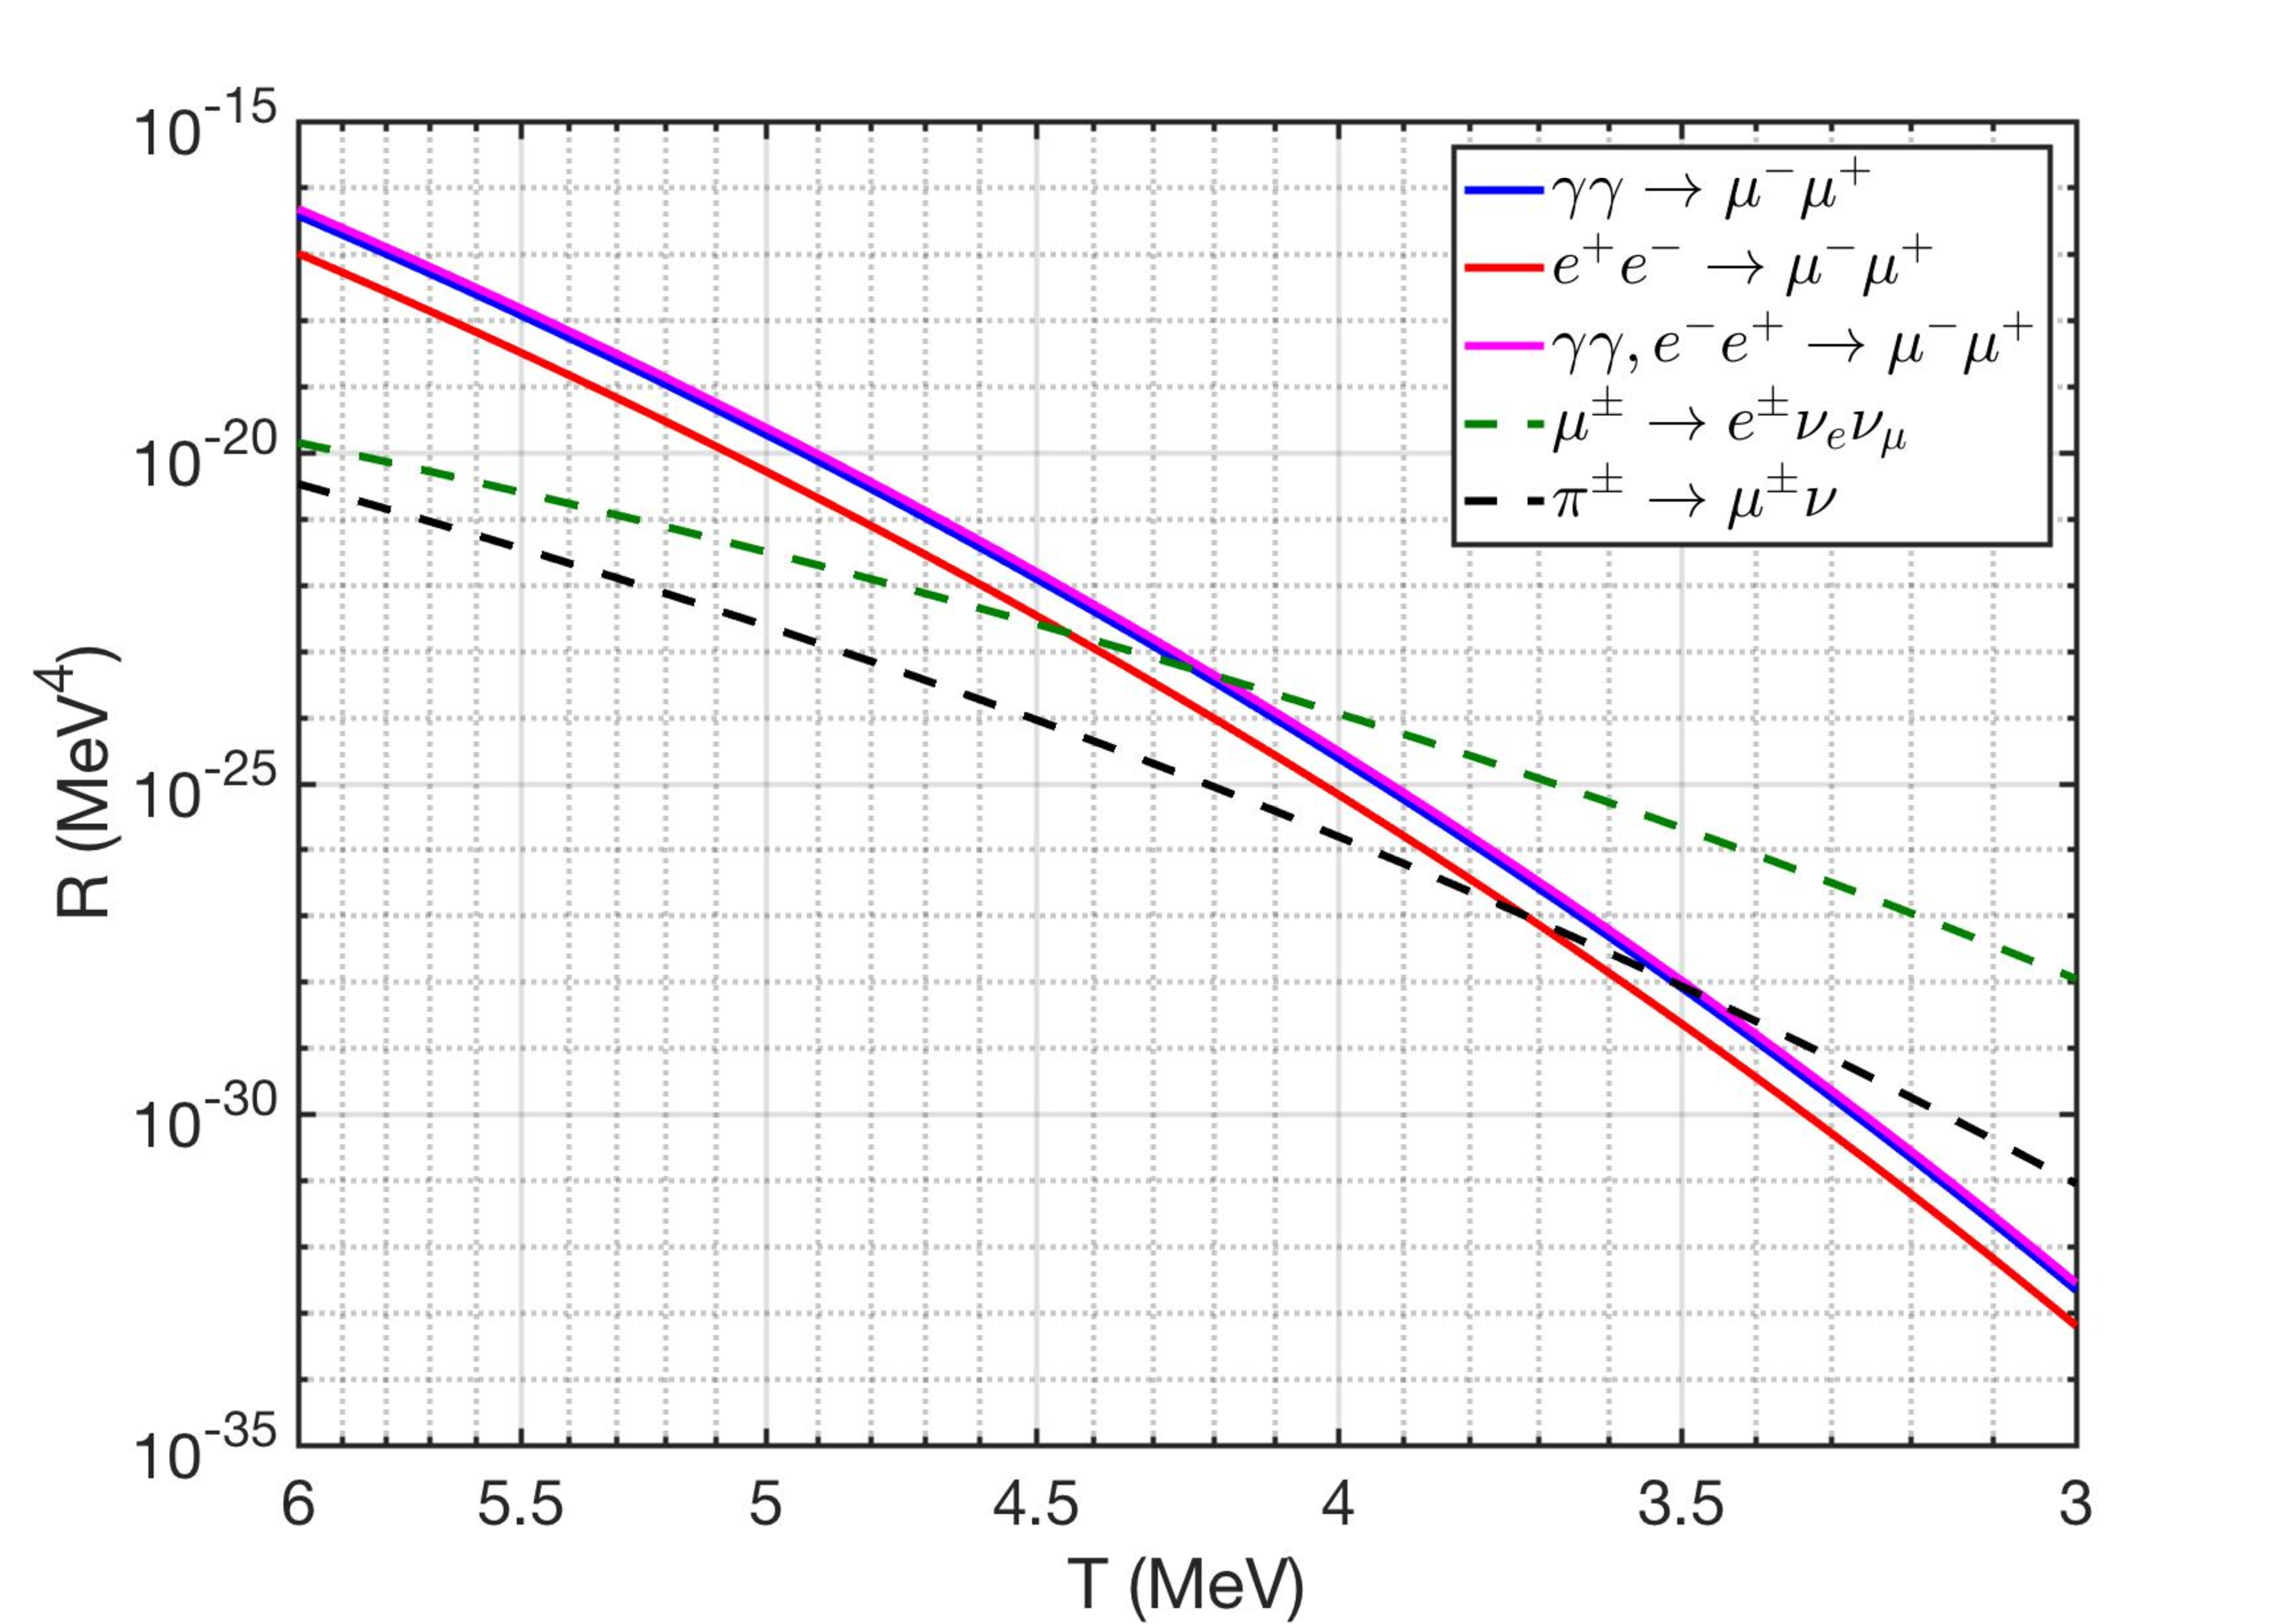
\includegraphics[width=5.0in]{./plots/MuonRate_new2.pdf}
\caption{We plot the thermal reaction rate per volume for different reactions as a function of temperature. We found that dominant reactions for $\mu^\pm$ production are ${\gamma+\gamma\to\mu^++\mu^-}$ and $e^++e^-\to\mu^++\mu^-$, and the total production rate crosses the decay rate of $\mu^\pm$ at temperature $T_{dissapear}\approx 4.195$ MeV.}
\label{MuonRatenew_fig}
\end{center}
\end{figure}
%~~~~~~~~~~~~~~~~~~~~~~~~~~~~~~~~~~~~~~~~~~~~~~~~~~~~~~~~~~~~~~~~~~~~~~~~~~~~~~~~~~~~~~~~~~~~~~~~

On the other hand, considering the number density for nonrelativistic $\mu^\pm$ in the Boltzmann approximation, we have
\begin{align}\label{nmupm}
n_{\mu^\pm}=\frac{g_{\mu^\pm}}{2\pi^2}T^3\left(\frac{m_\mu}{T}\right)^2 K_2(m_\mu/T)=g_{\mu^\pm}\left(\frac{m_\mu T}{2\pi}\right)^{3/2}e^{-{m_\mu}/{T}}\;. 
\end{align}
then the number density between $n_{\mu^\pm}$ and baryon $n_B$ can be written as
\begin{align}
\frac{n_{\mu^\pm}}{n_\mathrm{B}}=\frac{n_{\mu^\pm}}{s}\frac{s}{n_\mathrm{B}}=
\frac{n_{\mu^\pm}}{s}\left(\frac{s}{n_\mathrm{B}}\right)_{\!t_0},
\end{align}
where we used that $s/n_\mathrm{B}$ remains constant and $t_0$ represent present day value. The present value is given by $(n_B/s)_{t_0}\approx8.69\times10^{-11}$ (detail please see Chapter~\ref{Introduction}). The entropy density $s$ can be characterized introducing $g^s_\ast$, the total number of \lq entropic\rq\ degrees of freedom
\begin{align}\label{entrop}
s=\frac{2\pi^2}{45}g^s_\ast T^3\;.
\end{align}
For temperature $10\,\mathrm{MeV} >T>3 $\,MeV, the massless photons, nearly relativistic electron/positrons, and practically massless neutrinos contribute to the degree of freedom $g^s_\ast$.  In this case, the number density between $n_{\mu^\pm}$ and baryon $n_B$ in the temperature interval we consider $10\,\mathrm{MeV} >T>3 $\,MeV is given by
\begin{align}\label{nmuperbF} 
\frac{n_{\mu^\pm}}{n_\mathrm{B}}=\frac{45}{2\pi^2}\frac{g_{\mu^\pm}}{g^s_\ast}\left(\frac{m_\mu}{2\pi T}\right)^{3/2}e^{-{m_\mu}/{T}}\;\left(\frac{s}{n_\mathrm{B}}\right)_{\!t_0}.
\end{align}


%Figure~~~~~~~~~~~~~~~~~~~~~~~~~~~~~~~~~~~~~~~~~~~~~~~~~~~~~~~~~~~~~~~~~~~~~~~~~
\begin{figure}[t]
\begin{center}
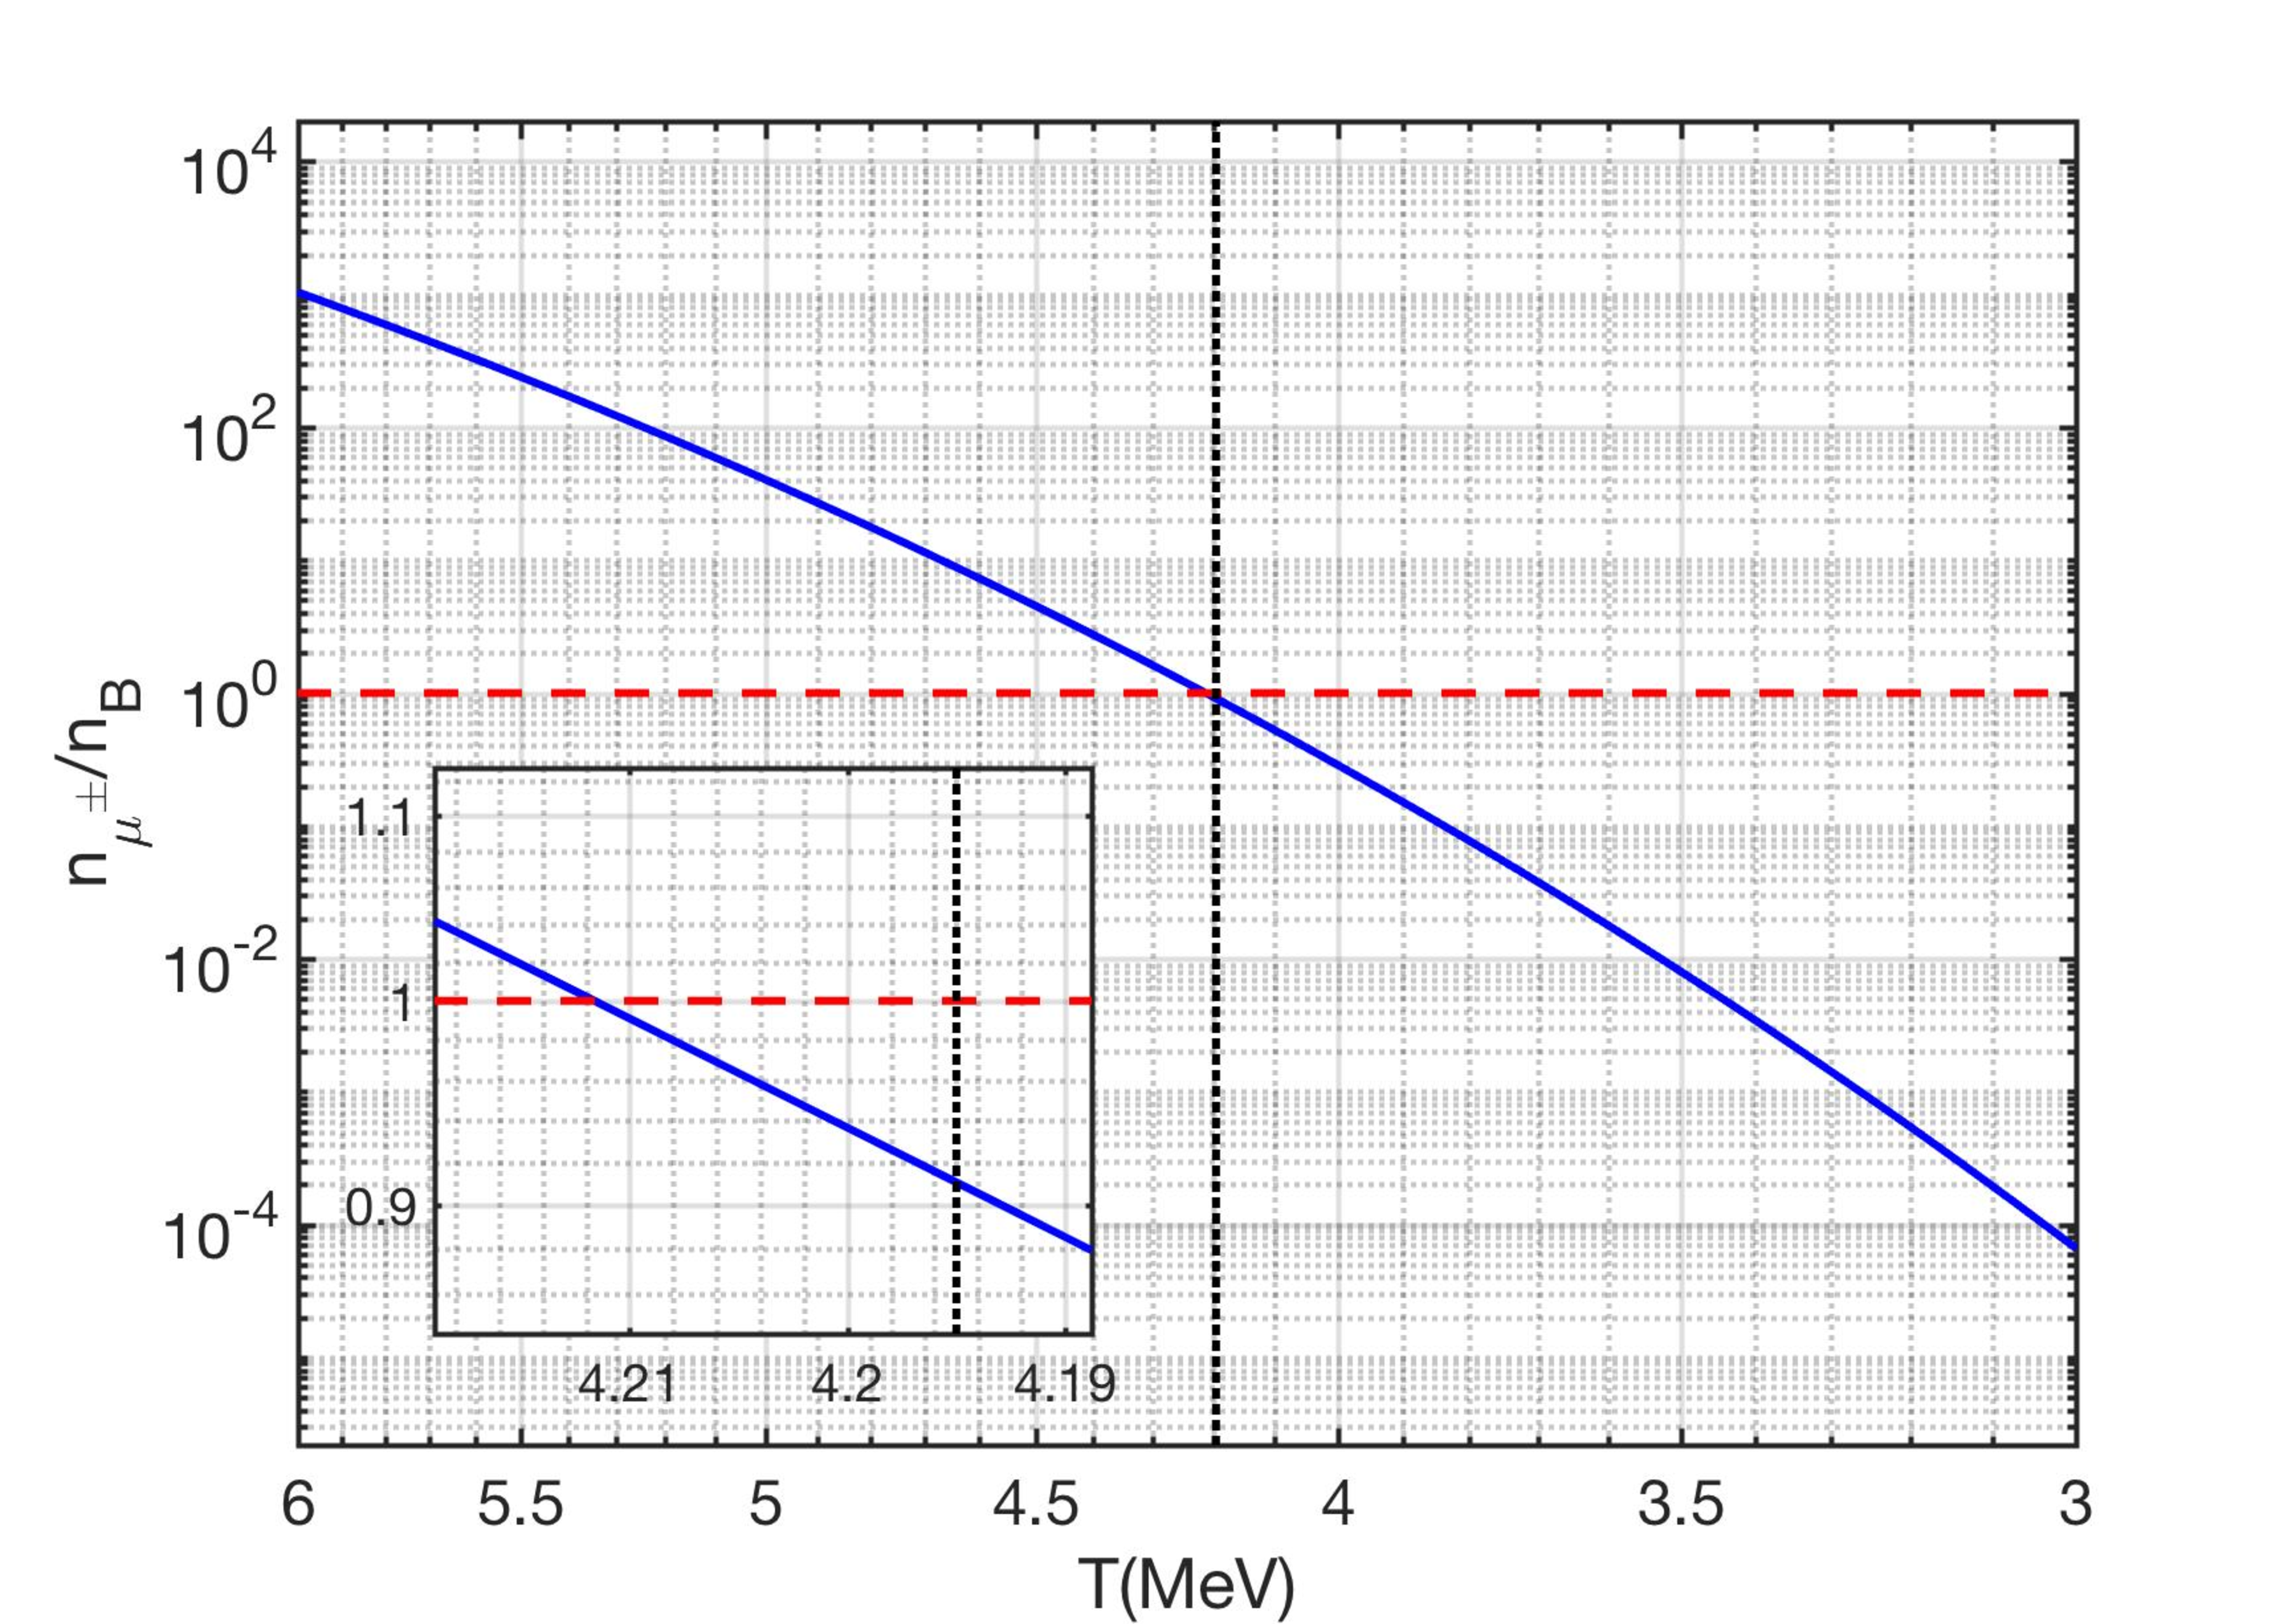
\includegraphics[width=\linewidth]{./plots/DensityRatio_new2.pdf}
\caption{
The density ratio between $\mu^\pm$ and baryons as a function of temperature. The density ratio at muon disappearance temperature is about $n_{\mu^\pm}/n_\mathrm{B}(T_\mathrm{disappear})\approx0.911$, and around the temperature $T\approx4.212$ MeV the density ratio $n_{\mu^\pm}/n_\mathrm{B}\approx1$.}
\label{DensityRatio_fig}
\end{center}
\end{figure}
%~~~~~~~~~~~~~~~~~~~~~~~~~~~~~~~~~~~~~~~~~~~~~~~~~~~~~~~~~~~~~~~~~~~~~~~~~~~~~


In Fig.\,\ref{DensityRatio_fig} we show the muon to baryon density ratio Eq.\,(\ref{nmuperbF}) as a function of $T$. We see that the muon abundance $T=10$\,MeV exceeds that of baryons by a factor 500,000 while at muon disappearance temperature $n_{\mu^\pm}/n_\mathrm{B}(T_\mathrm{disappear})\approx0.911$. The number density $n_{\mu^\pm}$ and $n_\mathrm{B}$  abundances are equal at around the temperature $T_\mathrm{equal}\approx4.212\,\mathrm{MeV} >  T_\mathrm{disappear}$.  This means that the muon abundance may still be able to influence baryon evolution because their number density is comparable to the baryon density.% However, we also find that at the temperature $T_\mathrm{equal}\approx4.212$\,MeV the density ratio is unity $n_{\mu^\pm}/n_\mathrm{B}\approx1$.

The primary insight of this work is that aside of protons, neutrons and other nonrelativistic particles, both positively and negatively charged muons $\mu^\pm$ are present in thermal equilibrium and in non-negligible abundance for $T>T_\mathrm{dissapear}\approx 4.195$\,MeV. This offers a new and tantalizing model building opportunity for anyone interested in baryon-antibaryon separation in the primordial Universe, strangelet formation, and perhaps other exotic primordial structure formation mechanisms.





%~~~~~~~~~~~~~~~~~~~~~~~~~~~~~~~~~~~~~~~~~~~~~~~~~

\section{ Electron-positron plasma in the early Universe}\label{section_electron}
%In this section we will focus on the following:
%\begin{itemize}
%    \item Chemical potential of electron in early universe
%    \item Electron-positron plasma in BBN (Damped sccreening)
%    \item Electron-positron magnetization
%%    \item Neutron Lifespan in magnetized electron/positron plasma.
%\end{itemize}

In the early Universe, after the neutrino freeze-out at $T\approx 2$\,MeV, the Universe is controlled by the electron-positron-photon plasma. In this section, we demonstrate the rich electron-positron plasma in the early Universe by examining the chemical potential $\mu_e$ in the charge-neutral and entropy-conserving Universe. We study the  microscope collision property of electron-positron plasma and explore the spin response of the electron-positron plasma to external and self-magnetization fields, thus developing methods for future detailed study.

%In this section, we will quantify the dynamical picture of $e^\pm$ plasma and show that the $e^+$ abundance can persist in early universe at relatively low temperature $T = 20$ keV which provide the dense $e^\pm$ plasma environment for the big-bang nucleosynthesis (BBN) in the early universe. 

%The role of electron-positron plasma has not received the appropriate attention in the days of precision big bang nucleosynthesis studies. The standard BBN model indicates that the synthesis of light elements typically takes place at temperatures around  $86\,\mathrm{keV}>T_{BBN}>50\,\mathrm{keV}$~[\cite{Pitrou:2018cgg}]. Within this temperature range there are millions of electron-positron pairs per charged nucleon, providing an electron-positron-rich plasma environment for nucleosynthesis. Furthermore, the electron-positron densities can reach millions of times normal atomic densities. The presence of  these $e\bar e$-pairs before and during BBN has been acknowledged by Wang, Bertulani and Balantekin~[\cite{Wang:2010px}] nearly a decade ago.





%On the other hand, the Universe today filled with magnetic fields at various scales and strengths both within galaxies and in deep extra-galactic space.It is currently unknown the origin for these magnetic fields today. In early Universe when temperature $T>20$ keV , we have dense $e^\pm$ plasma. The significant magnetic moments of electrons and positrons also provide opportunities to investigate spin magnetization process.


%~~~~~~~~~~~~~~~~~~~~~~~~~~~~~~~~~~~~~~~~~~~~~~~~~~~~~~~~~~~~~~~~~~~~~~~~~

\subsection{Electron chemical potential in the early Universe}
In this section, we derive the dependence of electron chemical potential, and hence $e^\pm$ density, on the photon background temperature by employing the following physical principles:
\begin{enumerate}
\item Charge neutrality of the Universe:
\begin{align}\label{neutrality}
n_e-n_{\overline{e}}=n_p-n_{\overline{p}}\approx\,n_p,
\end{align}
where $n_e$ and $n_{\overline{e}}$ denotes the number density of electron and positron.
\item Neutrinos decouple (freeze-out) at a temperature $T_f\simeq 2$ MeV, after which they free stream through the Universe with an effective temperature~[\cite{Birrell:2012gg}]
\begin{align}
T_\nu(t)=T_f a(t_f)/a(t),
\end{align}
 where $a(t)$ is the FLRW Universe scale factor.
\item Total comoving entropy is conserved. At $T\leq T_f$ the dominant contributors to entropy are photons, $e^\pm$, and neutrinos.
In addition, after neutrino freeze-out, neutrino comoving entropy is independently conserved ~[\cite{Birrell:2012gg}]. This  implies that the combined comoving entropy in $\gamma$, $e^\pm$ is also conserved for $T_\gamma\leq T_f$.
\end{enumerate}

Motivated by the fact that comoving entropy in $\gamma$, $e^\pm$ is conserved after neutrino freeze-out, we rewrite the charge neutrality condition, Eq.(\ref{neutrality}) in the form
\begin{align}\label{charge_neutral_cond2}
n_e-n_{\overline{e}}=X_p\frac{n_B}{s_{\gamma,e,\overline{e}}} s_{\gamma,e,\overline{e}},\qquad X_p\equiv\frac{n_p}{n_B},
\end{align}
where $n_B$ is the number density of baryons, and $s_{\gamma,e,\overline{e}}$ is the combined entropy density in photons, electrons, and positrons. During the Universe expansion, the comoving entropy and baryon number are conserved quantities, hence the ratio $n_B/s_{\gamma,e,\overline{e}}$ is conserved. We have
\begin{align}
\frac{n_B}{s_{\gamma,e,\overline{e}}}=\left(\frac{n_B}{s_{\gamma,e,\overline{e}}}\right)_{t_0}\!\!\!\!=\left(\frac{n_B}{s_{\gamma}}\right)_{t_0}\!\!\!\!=\left(\frac{n_B}{n_\gamma}\right)_{t_0}\left(\frac{n_\gamma}{s_{\gamma}}\right)_{t_0},
\end{align}
where the subscript $t_0$ denotes the present day value, and the second equality is obtained by observing that the present day $e^\pm$-entropy density is negligible compared to the photon entropy density. We can evaluate the ratio by giving the present day baryon-to-photon ratio: $n_B/n_\gamma= 6.05\times10^{-10}$(CMB) ~[\cite{ParticleDataGroup:2022pth}] and the entropy per particle for a massless boson:$(s/n)_{\mathrm{boson}}\approx 3.602$~[\cite{Letessier:2002ony}].

The total entropy density of photons and electron/positron can be written as
\begin{align}\label{entropy_per_baryon}
s_{\gamma,e,\overline{e}}=\frac{2\pi^2}{45}g_\gamma\,T_\gamma^3+\frac{\rho_{e,\overline{e}}+P_{e,\overline{e}}}{T_\gamma}-\frac{\mu_e}{T_\gamma}(n_e-n_{\overline{e}}),
\end{align}
where $ \rho_{e,\overline{e}}=\rho_{e}+\rho_{\overline{e}}$ and $P_{e,\overline{e}}=P_{e}+P_{\overline{e}}$ are the total energy density and pressure of electrons/positron respectively.
The energy density and pressure in electrons and positrons are given by
\begin{align}\label{rho_e}
\frac{\rho_{e,\overline{e}}}{T_\gamma^4}=\frac{g_e}{2\pi^2}M_e^4 \bigg[&\int_{1}^\infty \frac{ u^2\sqrt{ u^2-1} du}{\exp(M_e u-b_e)+1}+\int_{1}^\infty \frac{ u^2\sqrt{ u^2-1} du}{\exp(M_e u+b_e)+1}\bigg]\,,
\end{align}
and
\begin{align}\label{P_e}
\frac{P_{e,\overline{e}}}{T_\gamma^4}=\frac{g_e}{6\pi^2}M_e^4\bigg[&\int_{1}^\infty   \frac{(u^2-1)^{3/2} du}{\exp(M_e u-b_e)+1}+\int_{1}^\infty   \frac{(u^2-1)^{3/2} du}{\exp(M_e u+b_e)+1}\bigg],
\end{align}
where we introduce the dimensionless variables as follows: 
\begin{align}\label{Variables}
u=\frac{E}{m_e},\qquad M_e=\frac{m_e}{T_\gamma},\qquad b_e=\frac{\mu_e}{T_\gamma}.
\end{align}

By incorporating Eq.(\ref{charge_neutral_cond2}) and Eq.(\ref{entropy_per_baryon}), the charge neutrality condition can be expressed as
\begin{align}\label{charge_neutral_cond3}
&\left[1+X_p\left(\frac{n_B}{n_\gamma}\right)_{t_0}\left(\frac{n_\gamma}{s_{\gamma}}\right)_{t_0}\frac{\mu_e}{T_\gamma}\right]\frac{n_e-n_{\overline{e}}}{T_\gamma^3}\notag\\
&\qquad\qquad\qquad=X_p\left(\frac{n_B}{n_\gamma}\right)_{t_0}\left(\frac{n_\gamma}{s_{\gamma}}\right)_{t_0} \left(\frac{2\pi^2}{45}g_\gamma+\frac{\rho_{e,\overline{e}}+P_{e,\overline{e}}}{T_\gamma^4}\right).
\end{align}
Using the Fermi distribution, the number density of electrons over positrons in the early Universe is given by
\begin{align}\label{ee_density}
n_e-n_{\overline{e}}&=\frac{g_e}{2\pi^2}\left[\int_0^\infty\frac{p^2dp}{\exp{\left((E-\mu_e)\right)/T_\gamma}+1}\right.\left.-\int_0^\infty\frac{p^2dp}{\exp{\left((E+\mu_e)/T_\gamma\right)}+1}\right]\notag\\
&=\frac{g_e}{2\pi^2}{T_\gamma^3}\tanh(b_e)M_e^3\int_{1}^\infty \!\!\!\!\frac{  u \sqrt{u^2-1} du}{1+\cosh(M_eu)/\cosh(b_e)}.
\end{align}
Substituting Eq.(\ref{ee_density}) into Eq.(\ref{charge_neutral_cond3}) and giving the value of $X_p$, the charge neutrality condition can be solved to determine $\mu_e/T_\gamma$ as a function of $M_e$ and $T_\gamma$. 
%Fig~~~~~~~~~~~~~~~~~~~~~~~~~~~~~~~~~~~~~~~~~~~~~~~~~~~~~
\begin{figure}[ht]
\begin{center}
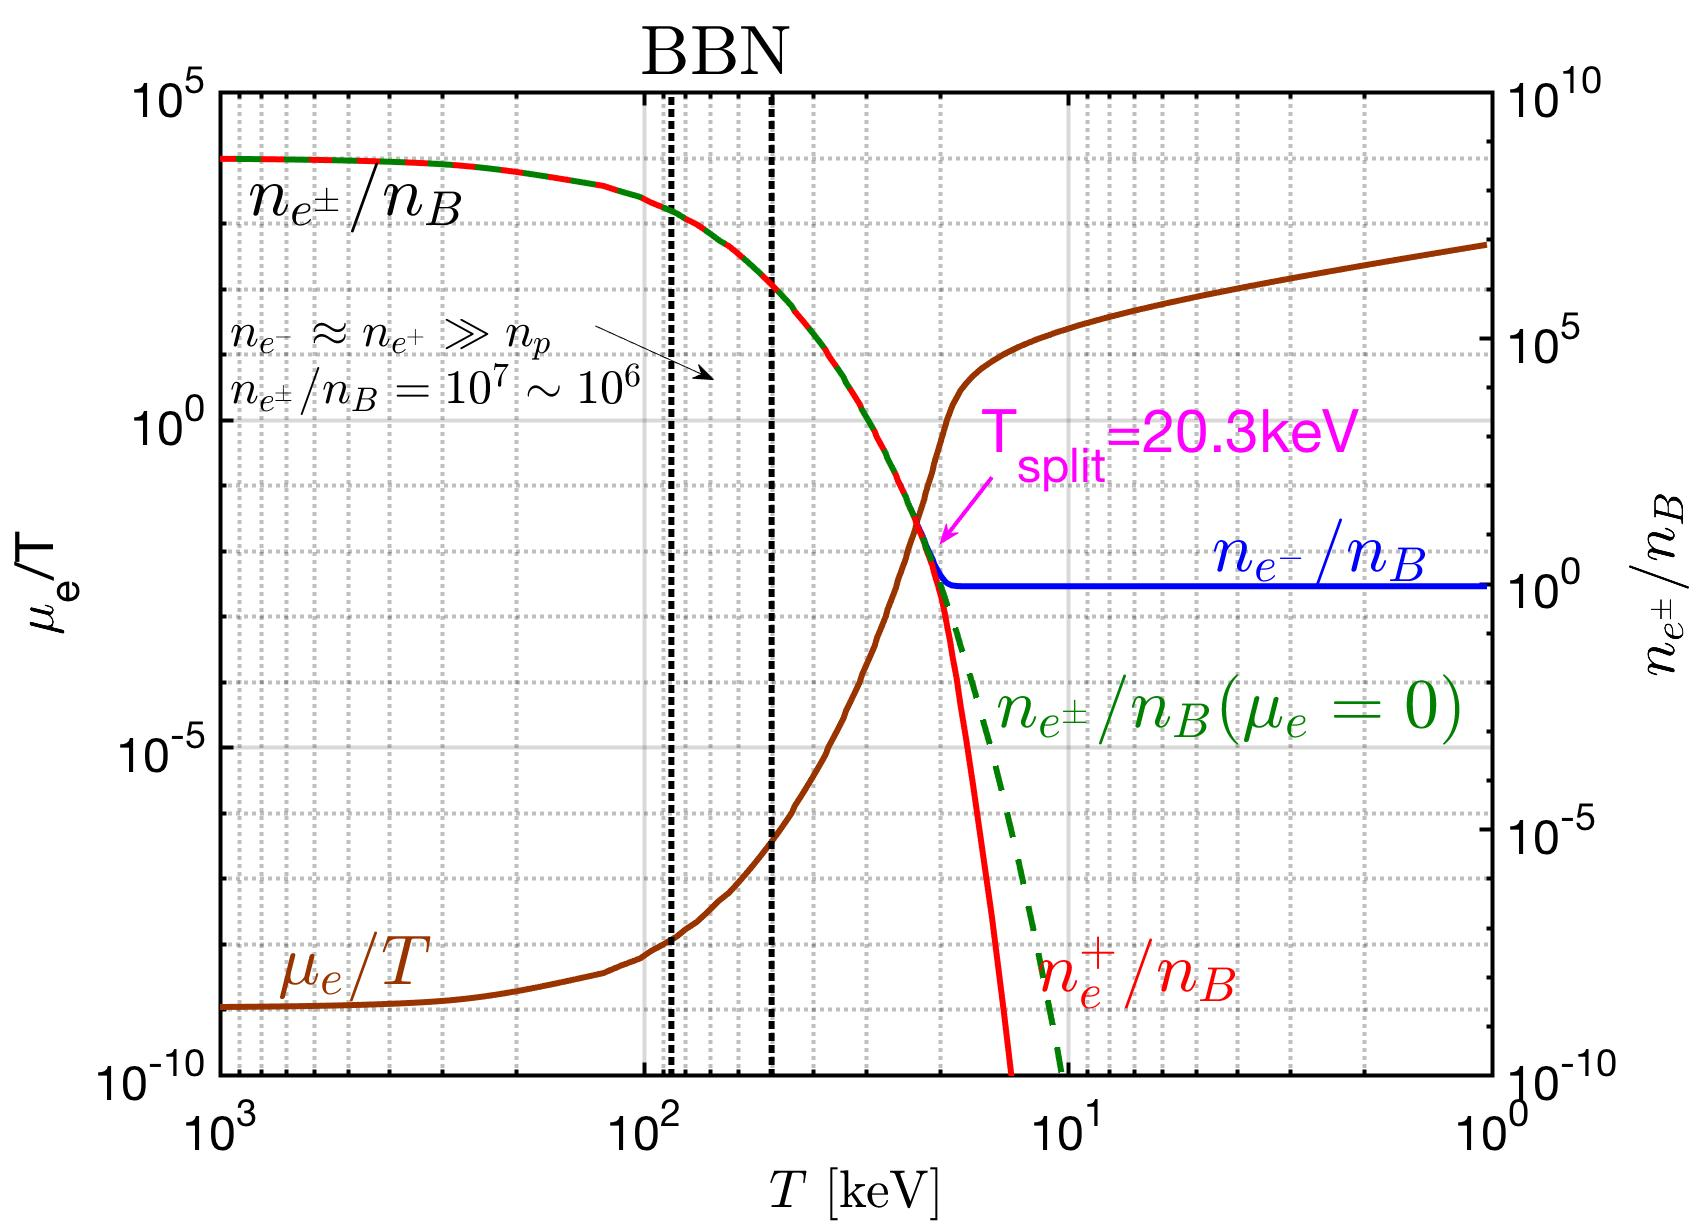
\includegraphics[width=\linewidth]{./plots/May152023_EPDensity_Chemical}
\caption{Left axis: The chemical potential of an electron as a function of photon temperature $T=T_\gamma$ with $X_p=0.878$ and $n_B/n_\gamma=6.05\times10^{-10}$. Right axis: the ratio of electron(positron) number density to baryon density as a function of temperature. The blue solid line is the electron density, the red dashed line is the positron density, and the green dotted line is the number density with $\mu_e=0$. We found that when electron chemical potential $\mu_e\approx T=0.02\,\mathrm{MeV}$ the positron density decreases because of the annihilation.}
\label{BBN_Electron}
\end{center}
\end{figure}
%~~~~~~~~~~~~~~~~~~~~~~~~~~~~~~~~~~~~~~~~~~~~~~~~~~~~~

In Fig.~\ref{BBN_Electron} (left axis) we solve Eq.(\ref{charge_neutral_cond3}) numerically and plot the electron chemical potential as a function of temperature with the following parameters: proton concentration $X_p=0.878$ from 
 observation~[\cite{ParticleDataGroup:2022pth}] and  $n_B/n_\gamma=6.05\times10^{-10}$ from CMB. We can see the value of chemical potential is comparatively small $\mu_e/T\approx10^{-6}\sim10^{-7}$ during the BBN temperature range, implying an equal number of electrons and positrons in plasma. From the ratio of electron (positron) number density to baryon density in Fig.~\ref{BBN_Electron} (right axis) we can see that during the accepted BBN temperature range the Universe was filled with an electron-positron rich plasma.
For example when the temperature is around $T=70\,\mathrm{keV}$ the density of electrons and positrons is comparatively large in the early Universe $n_{e^\pm}\approx10^7\,n_B$. Later when the temperature is around $T=20.3\,\mathrm{keV}$, the positron density decreases, leading to the transformation of the pair plasma to an electron-proton plasma.
%~~~~~~~~~~~~~~~~~~~~~~~~~~~~~~~~~~~~~~~~~~~~~~~~~
\subsection{Microscope damping rate of electron-positron plasma}\label{relax}
In electron-positron plasma, the major reactions between photons and $e^+e^-$ pairs are inverse Compton scattering, M{\o}ller scattering, and Bhabha scattering:
\begin{align}
&e^\pm+\gamma\longrightarrow e^\pm+\gamma,\qquad e^\pm+e^\pm\longrightarrow e^\pm+e^\pm,\qquad e^\pm+e^\mp\longrightarrow e^\pm+e^\mp.
\end{align}
The general formula for thermal reaction rate per volume is discussed in~[\cite{Letessier:2002ony}] (Eq.(17.16), Chapter 17). For inverse Compton scattering we have
\begin{align}
R_{e^{\pm}\gamma}=\frac{g_eg_\gamma}{16\left(2\pi\right)^5}T\int_{m_e^2}^\infty\!\!\!\!ds\frac{K_1(\sqrt{s}/T)}{\sqrt{s}}\int^0_{-(s-m_e^2)^2/s}\!\!\!\!\!\!\!\!\!\!\!\!\!\!\!\!dt\, |M_{e^{\pm}\gamma}|^2,
\end{align} 
and for M{\o}ller and Bhabha reactions we have
\begin{align}
&R_{e^\pm e^\pm}=\frac{g_eg_e}{16\left(2\pi\right)^5}T\!\!\int_{4m_e^2}^\infty\!\!\!\!ds\frac{K_1(\sqrt{s}/T)}{\sqrt{s}}\int^0_{-(s-4m_e^2)}\!\!\!\!\!\!\!\!\!\!\!\!\!\!\!\!dt\,|M_{e^\pm e^\pm}|^2,\\
&R_{e^\pm e^\mp}=\frac{g_eg_e}{16\left(2\pi\right)^5}T\!\!\int_{4m_e^2}^\infty\!\!\!\!ds\frac{K_1(\sqrt{s}/T)}{\sqrt{s}}\int^0_{-(s-4m_e^2)}\!\!\!\!\!\!\!\!\!\!\!\!\!\!\!\!dt\,|M_{e^\pm e^\mp}|^2,
\end{align}
where $g_i$ is the degeneracy of particle $i$, $|M|^2$ is the matrix element for a given reaction, $K_1$ is the Bessel function of order $1$, and $s,t,u$ are Mandelstam variables. The leading order matrix element associated with inverse Compton scattering can be expressed in the Mandelstam variables~[\cite{Kuznetsova:2011wt,Kuznetsova:2009bq}] we have
\begin{align}
|M_{e^\pm\gamma}|^2\!=32 \pi^2\alpha^2\bigg[&4\left(\frac{m_e^2}{m_e^2-s}+\frac{m_e^2}{m_e^2-u}\right)^2\notag\\
&\qquad\qquad-\frac{4m_e^2}{m_e^2-s}-\frac{4m_e^2}{m_e^2-u} -
 \frac{m_e^2-u}{m_e^2-s} -\frac{m_e^2-s}{m_e^2-u}\bigg],
\end{align}
and for M{\o}ller and Bhabha scattering we have 
\begin{align}
|M_{e^{\pm}e^{\pm}}|^{2}\!=64\pi^{2}\alpha^{2}\bigg[&
\frac{s^{2}+u^{2}+8m_e^{2}(t-m_e^{2})}{2(t-m^2_{\gamma})^{2}}\notag\\
&\quad+\frac{{s^{2}+t^{2}}+8m_e^{2}
(u-m_e^{2})}{2(u-m_{\gamma}^2)^{2}} + \frac{\left( {s}-2m_e^{2}\right)\left({s}-6m_e^{2}\right)}
{(t-m_{\gamma}^2)(u-m_{\gamma}^2)} \bigg],
\end{align}
and
\begin{align}
|M_{e^\pm e^\mp}|^{2}=64\pi^{2}\alpha^{2}
\bigg[&\frac{s^{2}+u^{2}+8m_e^{2}(t-m_e^{2})}{2(t-m^2_{\gamma})^{2}}\notag\\
&\quad+\frac{u^{2}+t^{2}+8m_e^{2}
(s-m_e^{2})}{2(s-m^2_{\gamma})^{2}}  +   \frac{\left({u}-2m_e^{2}\right)\left({u}-6m_e^{2}\right)}
   {(t-m^2_{\gamma})(s-m^2_{\gamma})} \bigg],
\label{M_fi_b}
\end{align}
where we introduce the photon mass $m_\gamma$ to account the plasma effect and avoid singularity in reaction matrix elements. 

The photon mass $m_\gamma$ in plasma is equal to the plasma frequency $\omega_p$, where we have~[\cite{Kislinger:1975uy}]
\begin{align}
m^2_\gamma=\omega^2_{p}=8\pi\alpha\int\frac{d^3p_e}{(2\pi)^3}\left(1-\frac{p_e^2}{3E_e^2}\right)\frac{f_e+f_{\bar e}}{E_e},
\end{align}
where $E_e=\sqrt{p_e^2+m^2_e}$. In the BBN temperature range $86\,\mathrm{keV}>T_{BBN}>50\,\mathrm{keV}$ we have $m_e\gg T$ and considering the nonrelativistic limit for electron-positron plasma, we obtain
\begin{align}
m^2_\gamma=\frac{4\pi\alpha}{2m_e}\left(\frac{2m_eT}{\pi}\right)^{3/2}e^{-m_e/T}\cosh\left(\frac{\mu_e}{T}\right).
\end{align}
In the BBN temperature range, we have $\mu_e/T\ll1$, which implies the equal number of electrons and positrons in plasma.

To discuss the collisional plasma by the linear response theory, it is convenient to define the average relaxation rate for the electron-positron plasma as follows:
\begin{align}\label{Kappa}
\kappa=\frac{R_{e^\pm e^\pm}+R_{e^\pm e^\mp}+R_{e^\pm\gamma}}{\sqrt{n_{e^-}n_{e^+}}}\approx\frac{R_{e^\pm e^\pm}+R_{e^\pm e^\mp}}{\sqrt{n_{e^-}n_{e^+}}},
\end{align}
where the density function ${\sqrt{n_{e^-}n_{e^+}}}$ in the Boltzmann limit is given by
\begin{align}
{\sqrt{n_{e^-}n_{e^+}}}=\frac{g_e}{2\pi^3}T^3\left(\frac{m_e}{T}\right)^2K_2(m_e/T).
\end{align}
In Fig.~\ref{RelaxationRate_fig}, we show the reaction rates for M{\o}ller reaction, Bhabha reaction, and inverse Compton scattering as a function of temperature. For temperatures $T>12.0$ keV, the dominant reactions in plasma are M{\o}ller and Bhabha scatterings between electrons and positrons. Thus in the BBN temperature range, we can neglect the inverse Compton scattering. The total relaxation rate is approximately constant $\kappa=10\sim12$ keV during the BBN. For $T<20.3$ keV the relaxation rate $\kappa$ decreases rapidly because of positron annihilation. At this temperature, the composition of plasma begins to change from an electron-positron plasma to an electron-baryon plasma.
%~~~~Figure~~~~~~~~~~~~~~~~~~~~~~~~~~~
\begin{figure}[h]
\begin{center}
%\includegraphics[width=0.95\linewidth]{KappaRateToT_May082023}
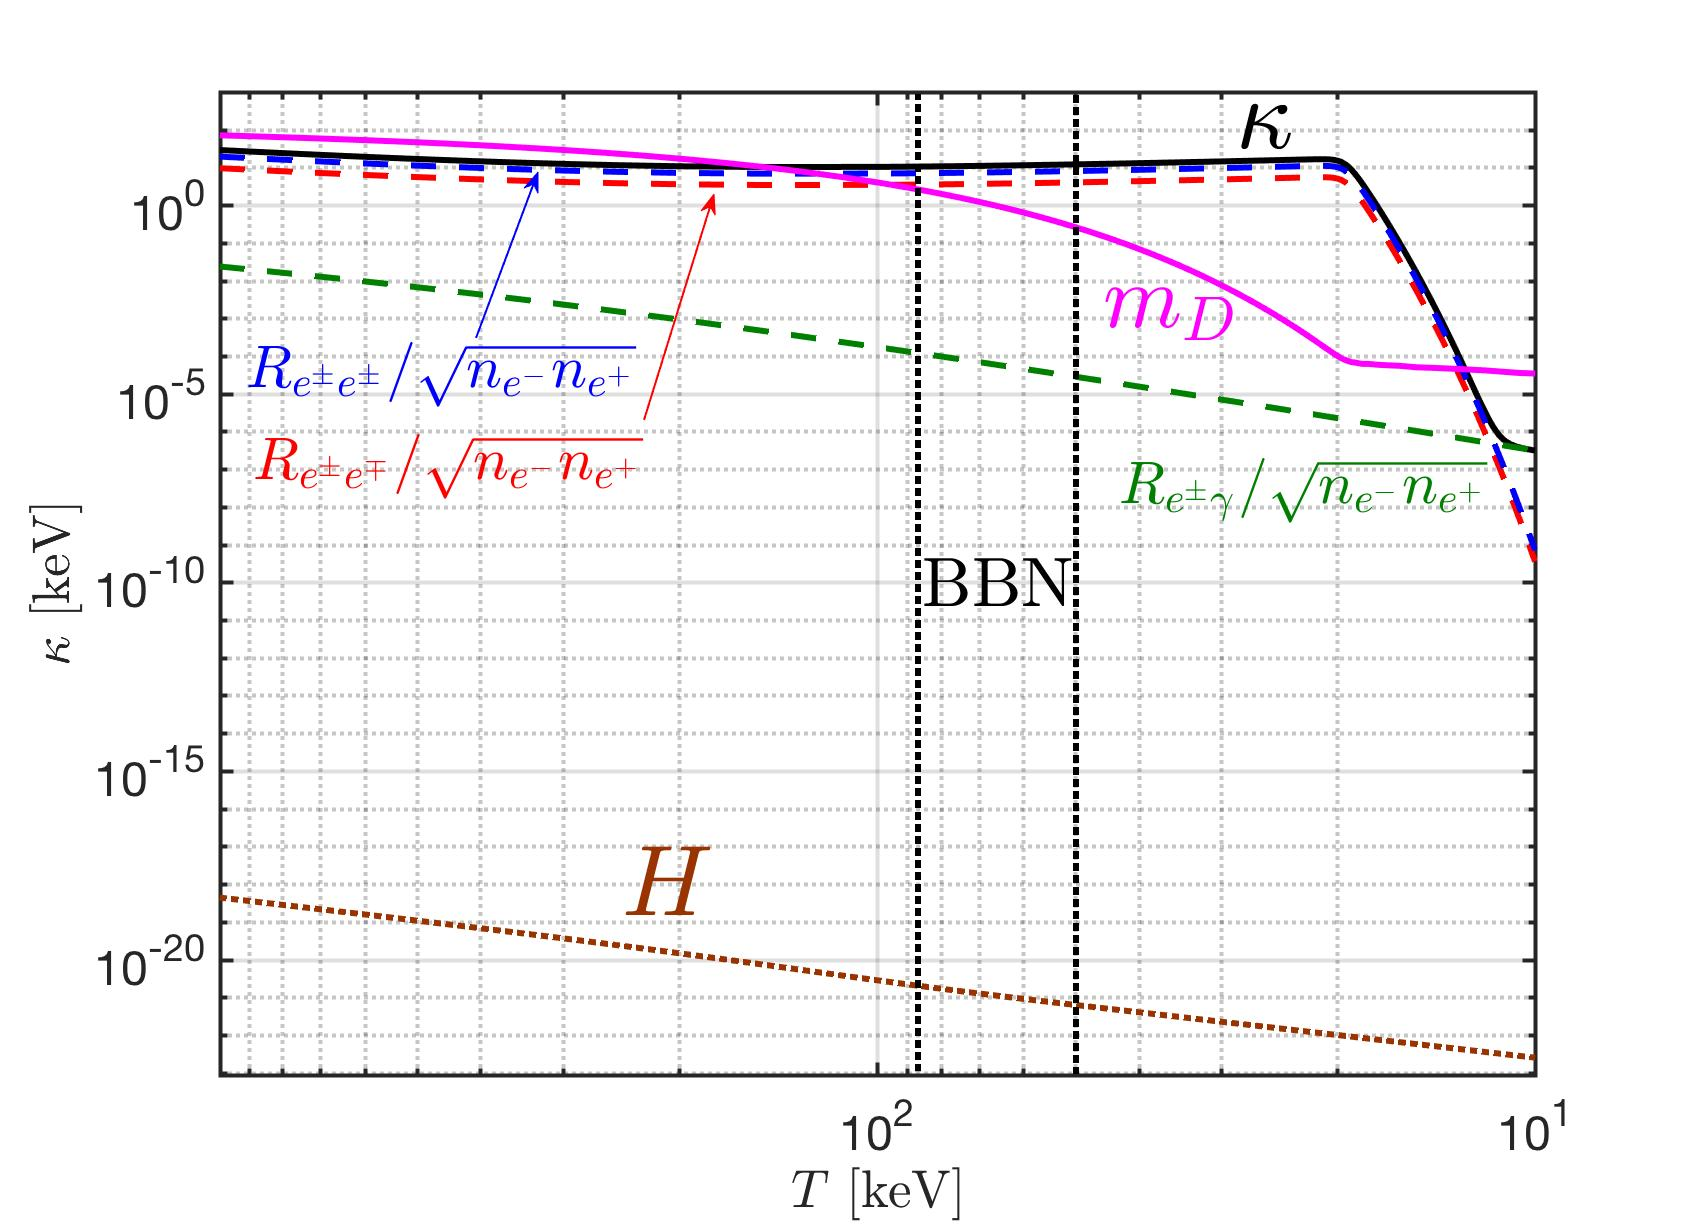
\includegraphics[width=\linewidth]{./plots/May152023Kappa_EPPlasma}
\caption{The relaxation rate $\kappa$ as a function of temperature in nonrelativistic electron-positron plasma. For comparison, we show  reaction rates  for M{\o}ller reaction $e^-+e^-\to e^-+e^-$ (blue line), Bhabha reaction $e^-+e^+\to e^-+e^+$ (red line), and inverse Compton scattering $e^-+\gamma\to e^-+\gamma$ (green line) respectively. It shows that the dominant reactions during BBN are the M{\o}ller and Bhabha scatterings between electrons and positrons. The total relaxation rate Eq.(\ref{Kappa}) is shown in the black line. It shows that we have $\kappa=10\sim12$ keV during the BBN temperature range. For comparison, the Debye mass $m_D=\omega_{p}\sqrt{m_e/T}$(purple line) is shown as a function of temperature.
}
\label{RelaxationRate_fig}
\end{center}
\end{figure}
%~~~~Figure~~~~~~~~~~~~~~~~~~~~~~~~~~~


\subsubsection{From static to damped dynamic screening}

At present, the observation of light element (e.g. D, $^3$He, $^4$He, and $^7$Li) abundances produced in Big-Bang nucleosynthesis (BBN) offers a reliable probe of the early Universe before the recombination. Much effort of the BBN study is currently being made to reconcile the discrepancies and tensions between theoretical predictions and observations of light element abundances, e.g. $^7$Li problem ~[\cite{Pitrou:2018cgg,Fields:2011zzb}].
Current models assume that the Universe was essentially void of anything but reacting light nucleons and electrons needed to keep the local baryon density charge-neutral, a situation similar to the experimental environment where empirical nuclear reaction rates are obtained.

The electron-positron plasma influences light element abundances through electromagnetic screening of the nuclear potential. The electron cloud surrounding the charge of an ion screens other nuclear charges far from its own radius and reduces the Coulomb barrier. In nuclear reactions, the reduction of Coulomb barrier makes the penetration probability easier and enhance the thermonuclear reaction rates. In this case, the modification of the nuclei interaction due to the plasma screening effect may plays a key role in the formation of light element in the BBN. 

The enhancement factor of thermonuclear reaction rates and screening potential are calculated by Salpeter in 1954~[\cite{Salpeter:1954nc}], which describes the static screening effects for the thermonuclear reactions. In an isotropic and homogeneous plasma the Coulomb potential of a point-like particle with charge $Ze$ at rest is modified into~[\cite{Salpeter:1954nc}]
\begin{align}
\phi_\text{stat}(r)=\frac{Ze}{4\pi\epsilon_0 r}e^{-m_Dr},
\end{align}
where $m_D$ is the Debye mass. After that it has been exploited widely in BBN for static screening ~[\cite{1969ApJ...155..183S,Famiano:2016hhs}]. 

Subsequently, the study of dynamical screening for moving ions has been taken into account~[\cite{1988ApJ...331..565C,Gruzinov:1997as,Hwang:2021kno}]. When a test charge moves with a velocity that is enough to react with the background charge in plasma, the Coulomb potential is modified by the dynamical effect. However, the applications focus on the weakly interacting electron-positron plasma only. 

In our separate work~[\cite{Grayson:2023flr}] we use the linear response theory adapted by C.Grayson to to describe the inter nuclear potential in electron-positron plasma during BBN. We improve the prior efforts by evaluation and inclusion of the collision damping rate due to scattering in the dense plasma medium and provide an approximate analytic formula that can be readily used to estimate the effect of screening on internuclear potential. For comprehensive discussion and the application of the damped dynamic screening see~[\cite{Grayson:2023flr}].










%~~~~~~~~~~~~~~~~~~~~~~~~~~~~~~~~~~~~~~~~~~~~~~~~~~~~
\subsection{Magnetization of the electron-positron plasma}

In the present-day Universe, we have magnetic fields~\cite{Giovannini:2003yn,Kronberg:1993vk} at various scales and strengths both within galaxies and in deep extra-galactic space far away from matter sources. Current observations suggest the upper and lower bounds for the Extra-Galactic Magnetic Field (EGMF) are given by~[\cite{neronov2010evidence,taylor2011extragalactic,pshirkov2015new,jedamzik2019stringent,vernstrom2021discovery}]
\begin{align}
    \label{egmf}
    10^{-8}{\mathrm G}>B_{\mathrm{EGFM}}>10^{-16}{\mathrm G}\,.
\end{align}
The origin for EGMF today is currently unknown; different models are considered in lectures~[\cite{Widrow:2011hs,Vazza:2021vwy}]. In our work~[\cite{Rafelski:2023emw}], we investigate the hypothesis that the observed EGMF are primordial in nature, predating even the recombination
epoch. Under this hypothesis, the first best candidate is the electron-positron plasma. This is because for the temperature range $ 200\,\mathrm{keV} > T > 20$ keV, we still have relatively large quantity of both $e^\pm$ in the the early Universe plasma. In addition, electrons and positrons have the largest magnetic moments in nature, are likely to have been magnetized in the early Universe due to spin orientation. These  provide the possibility origins for a primordial magnetic field.

As the Universe undergoes the isentropic expansion,  the temperature gradually decreases as $T\propto1/a(t)$, where $a(t)$ represents the scale factor. The assumption is made that the magnetic flux is conserved over comoving surfaces, implying that the primordial relic field is expected to dilute as $B\propto1/a(t)^{2}$~[\cite{Rafelski:2023emw}]. Combining these cosmological redshift relations, we can introduce a dimensionless cosmic magnetic scale that remains unchanged during the evolution of the Universe 
\begin{align}
    \label{tbscale}
    b \equiv\frac{e{B}}{T^{2}}=\left(\frac{e{B}}{T^{2}}\right)_{t_0}=b_0={\rm\ const.}\qquad10^{-3}>b_{0}>10^{-11}\,.
\end{align}
The upper and lower bounds for $b_0$ are estimated by using the present day EGMF observations Eq.~(\ref{egmf}) and the present CMB temperature $T_{0}=2.7\,\mathrm{K}\approx2.3\times10^{-4}$ eV~[\cite{aghanim2018planck}].
As $b_0$ is a constant of expansion, this means the contemporary small bounded values of may have once represented large magnetic fields in the early Universe and require detailed study in a different epoch of the Universe. Therefore, correctly describing the dynamics of this $e^{\pm}$ plasma is of interest when considering the origin of extra-galactic magnetic fields (EGMF). 

In the following,  we will demonstrate that fundamental quantum statistical analysis can lead to further insights on the behavior of magnetized plasma, and show that the $e^\pm$ plasma is overall paramagnetic and yields a positive overall magnetization, which
is contrary to the traditional assumption that matter-antimatter plasma lack significant magnetic responses. For more detailed discussion  of electron-positron plasma magnetization, please see~[\cite{Andrew:2023abc}].



\subsubsection{Electron-positron partition function}
To study the statistical behavior of the $e^\pm$ system in a magnetic field, we utilize the general Fermion partition function~[\cite{Elze:1980er}]
\begin{align}
 \label{PartFunc} \ln\mathcal{Z}=\sum_{\alpha}\ln\left(1+e^{-\beta(E-\eta)}\right)\,,
\end{align}
where $\beta=1/T$, $\alpha$ is the set of all quantum numbers in the system, and $\eta$ is the generalized chemical potential. In the case of a magnetized $e^{\pm}$ system, we consider it as a system of four quantum species: Particles and antiparticles, and spin aligned and anti-aligned. Taken together, we consider a system where electrons and positrons can be spin aligned or anti-aligned with the magnetic field $B$ and the partition function of the system can be written as
\begin{align}\label{PartFuncB}
%&\ln\mathcal{Z}_{tot}=&\frac{2eBV}{(2\pi)^2}\sum_{\sigma}^{\pm1}\sum_{s}^{\pm1/2}\sum_{n=0}^\infty\int^\infty_{0}dp_z\left[\ln\left(1+\Upsilon_{\sigma}^{s}(x)e^{-\beta E_{n}^{s}}\right)\right]\,\\
\ln\mathcal{Z}_{tot}=\frac{2eBV}{(2\pi)^2}\sum_{\sigma}^{\pm1}\sum_{s}^{\pm1/2}\sum_{n=0}^\infty\int^\infty_{0}dp_z\left[\ln\left(1+\Upsilon(x)e^{(\sigma\eta_{e}+s\eta_s)/T}e^{-\beta E_{n}^{s}}\right)\right]\,,
\end{align}
where $n$ is the principle quantum number for the Landau levels. The parameter $\eta_{e}$ is the electron chemical potential and $\eta_s$ is the spin chemical potential~[\cite{Andrew:2023abc}]. The parameter $\Upsilon(x)$ is the fugacity of the Fermi gas. In this thesis we will focus on the case $\Upsilon(x)=1$ and $\eta_s=0$ , 
we leave the general case $\Upsilon(x)\neq1$ and $\eta_s\neq0$ for future work.



%In general, $\Upsilon=1$ represents the maximum entropy and corresponds to the normal Fermi distribution. The deviation of $\Upsilon\neq1$ represents the configurations of reduced entropy without pulling the system off a thermal temperature. This scenario is well studied for quarks in QGP. The situation for $e^\pm$ plasma is similar to the case of the quarks during QGP, but instead here the deviation is spatial rather than temporal. Inhomogeneity can arise from the influence of other forces on the gas such as gravitational forces. This is precisely the kind of behavior that may arise in the $e^{\pm}$ epoch as the dominant photon thermal bath keeps the Fermi gas in thermal equilibrium while spatial inequilibrium could spontaneously develop. 


In the following, we will retain $\Upsilon(x)=1$ and consider the case $\eta_s/T\ll1$ for the first approximation. Then the partition function becomes
\begin{align}
\ln\mathcal{Z}_{tot}=\frac{2eBV}{(2\pi)^2}\sum_{s}^{\pm1/2}\sum_{n=0}^\infty\int^\infty_{0} \!\!dp_z\bigg[\ln\left(1+e^{-\beta(E_{n}^s-\eta_e)}\right)+\ln\left(1+e^{-\beta(E_{n}^s+\eta_e)}\right)\bigg].
\end{align}
Considering the $e^\pm$ plasma in a uniform magnetic field $B$ pointing along the $z$-axis, the energy $E_{n}^\pm$ of electron/positron system can be written as~[\cite{Rafelski:2023emw}]
\begin{align}
&E_{n}^\pm=\sqrt{p^2_z+\tilde m^2_\pm+2eBn},\qquad\tilde{m}^2_\pm=m^2_e+eB\left(1\mp\frac{g}{2}\right)\,,
\end{align}
where the $\pm$ script refers to spin aligned and anti-aligned eigenvalues. The parameter $g$ is the gyro-magnetic ($g$-factor) of the particle. 

To simplify the partition function, we consider the expansion of the logarithmic function as follows:
\begin{align}
\ln\left(1+x\right)=\sum^{\infty}_{k=1}\frac{(-1)^{k+1}}{k}x^k, \,\,\,\,\,\,\,\mathrm{for}\,|x|<1.
\end{align}
Then the partition function of electron/positron system can be written as
\begin{align}
\ln\mathcal{Z}_{tot}=&\frac{2eBV}{(2\pi)^2}\sum_{n=0}^\infty\int^\infty_{0} \!\!dp_z\sum^{\infty}_{k=1}\frac{(-1)^{k+1}}{k}\bigg[e^{k\beta\mu_e}+e^{-k\beta\mu_e}\bigg]e^{-k\beta E_n^\pm}\notag\\
&=\frac{2eBV}{(2\pi)^2}\sum_{n=0}^\infty\sum^{\infty}_{k=1}\frac{(-1)^{k+1}}{k}\bigg[2\cosh{(k\beta\mu_e)}\bigg]\int_0^\infty dp_z\,e^{-k\beta E_n^\pm}.
\end{align}
Using the general definition of Bessel function:
\begin{align}
K_\nu(\beta m)=\frac{\sqrt{\pi}}{\Gamma({\nu-1/2})}\frac{1}{m}\left(\frac{\beta}{2m}\right)^{\nu-1}\int_0^\infty\,dp\,p^{2\nu-2}e^{-\beta E} \,\,\,\,\,\,\,\mathrm{for}\,\nu>1/2,
\end{align}
the integral over $dp_z$ can be written as
\begin{align}
\int_0^\infty dp_z\,e^{-k\beta E_n^\pm}&=\frac{\Gamma{(1/2)}}{\sqrt{\pi}}\sqrt{\tilde{m}^2_\pm+2eBn}\,\,K_1\!\!\left({k\sqrt{\tilde{m}^2_\pm+2eBn}}/{T}\right)\notag\\&=\sqrt{\tilde{m}^2_\pm+2eBn}\,\,K_1\!\!\left({k\sqrt{\tilde{m}^2_\pm+2eBn}}/{T}\right).
\end{align}
In this case, the partition function becomes
\begin{align}
\ln\mathcal{Z}_{tot}&=\frac{2eBV}{(2\pi)^2}\sum_{n=0}^\infty\sum^{\infty}_{k=1}\frac{(-1)^{k+1}}{k}\bigg[2\cosh{(k\beta\mu_e)}\bigg]\sqrt{\tilde{m}^2_\pm+2eBn}\,\,K_1({k\sqrt{\tilde{m}^2_\pm+2eBn}}/{T})\notag\\
&=\frac{2eBTV}{(2\pi)^2}\sum^{\infty}_{k=1}\frac{(-1)^{k+1}}{k^2}\bigg[2\cosh{(k\beta\mu_e)}\bigg]\sum_{n=0}^\infty W^\pm_1(n),
\end{align}
where we introduce the function $W^\pm_1(n)$ as follows
\begin{align}
W^\pm_1(n)\equiv\frac{k\sqrt{\tilde{m}^2_\pm+2eBn}}{T}\,\,K_1\!\!\left({k\sqrt{\tilde{m}^2_\pm+2eBn}}/{T}\right).
\end{align}

Considering the Euler-Maclaurin formula to replace the sum over Landau levels, we have
\begin{align}
\sum^{\infty}_{n=0}W^\pm_1(n)=\int^\infty_0\!\!dn\,W^\pm_1(n)&+\frac{1}{2}\bigg[W^\pm_1(\infty)+W^\pm_1(0)\bigg]\notag\\
&\qquad+\frac{1}{12}\bigg[\left.\frac{\partial W^\pm_1}{\partial n}\right|_{\infty}-\left.\frac{\partial W^\pm_1}{\partial n}\right|_{0}\bigg]+R,
\end{align}
where $R$ is the error remainder which is defined by integrals over Bernoulli polynomials which is small and can be neglected~[\cite{Elze:1980er}]. Using the properties of Bessel function we have
\begin{align}
&\frac{\partial W^\pm_1}{\partial n}=-\frac{k^2eB}{T^2}K_0\left({k\sqrt{\tilde{m}^2_\pm+2eBn}}/{T}\right),\qquad W^\pm_1(\infty)=0,\\
&\int^\infty_a\!\!dx\,x^2K_1(x)=a^2K_2(a),
\end{align}
then we obtain
\begin{align}
\sum^{\infty}_{n=0}W^\pm_1(n)
&=\left(\frac{T^2}{k^2eB}\right)\left[\left(\frac{k\tilde{m}_\pm}{T}\right)^2K_2(k\tilde m_\pm/T)\right]+\frac{1}{2}\left[\left(\frac{k\tilde{m}_\pm}{T}\right)K_1(k\tilde m_\pm/T)\right]\notag\\
&\qquad+\frac{1}{12}\left[\left(\frac{k^2eB}{T^2}\right)K_0(k\tilde m_\pm/T)\right].
\end{align}
Replacing the sum over Landau levels by the integral, the partition function becomes
\begin{align}
\ln\mathcal{Z}_{tot}=\ln\mathcal{Z}_{free}+\ln\mathcal{Z}_B\,,
\end{align}
where we define the partition functions as  
\begin{align}
 \label{FreePart}&\ln\mathcal{Z}_{free}=\frac{T^3V}{2\pi^2}\left[2\cosh{\left(\frac{\eta_{e}}{T}\right)}\right]\sum_{i=\pm}x_i^2K_2\left(x_i\right)\,,\qquad x_i=\frac{\tilde{m}_i}{T}\\
 \label{MagPart}&\ln\mathcal{Z}_B=\frac{eBTV}{2\pi^2}\left[2\cosh{\left(\frac{\eta_{e}}{T}\right)}\right]\sum_{i=\pm}\bigg[\frac{x_i}{2}K_1\left(x_i\right)+\frac{b_0}{12}K_0\left(x_i\right)\bigg]\,.
\end{align}
The partition function $\ln(\mathcal{Z}_{free})$ in Eq.~(\ref{FreePart}) represents the general form of the Fermi partition function for $e^\pm$ with "effective mass" $\tilde{m}_\pm$ in our system. When the magnetic field $B=0$ the function $\ln(\mathcal{Z}_{free})$ will go back to the general form of the Fermi partition function without the external field. The partition function $\ln\mathcal{Z}_B$ gives us the partition with magnetic field effect to the order  $\mathcal{O}(eB)$ and  $\mathcal{O}(eB)^2$.


In the temperature domain $ 200\,\mathrm{keV} > T > 20$ keV, we have $m_e\gg T$, and it suffices to consider the Boltzmann limit of the quantum distributions. Considering the Boltzmann approximation for non-relativistic electrons and positrons we can rewrite Eq.~(\ref{FreePart}) - Eq.~(\ref{MagPart}) and obtain
\begin{align}
 \label{lnZ}
&\ln\mathcal{Z}_{tot}\!=\!\frac{T^3V}{2\pi^2}\left[2\cosh\left(\frac{\eta_{e}}{T}\right)\right]\sum_{i=\pm}\left\{x_i^{2} K_2\left(x_i\right)+\frac{b_0}{2}x_iK_1\left(x_i\right)+\frac{b^2_0}{12}K_0\left(x_i\right)\right\}.
\end{align}
Given the partition function Eq.~(\ref{lnZ}), we can explore the chemical potential and magnetization of $e^\pm$ plasma in the early Universe
under the hypothesis of charge neutrality and entropy conservation.

\subsubsection{Electron chemical potential under magnetic field}
We explore the chemical potential of electron-positron plasma in a uniform magnetic field $B$ in the early Universe under the hypothesis of charge neutrality and entropy conservation. Considering the temperature after neutrino freeze-out, the charge neutrality condition can be written as
\begin{align}
 \label{density_proton}
 \left(n_{e}-n_{\bar{e}}\right)=n_{p}=X_p\,\left(\frac{n_{B}}{s_{\gamma,e}}\right)\,s_{\gamma,e},\qquad X_p\equiv\frac{n_p}{n_B}\,,
\end{align}
where $n_{p}$ and $n_B$ is the number density of protons and baryons respectively. Using the partition function Eq.~(\ref{lnZ}), the net number density of electrons in Boltzmann approximation can be written as
\begin{align}\label{NetElectron}
\left(n_e-n_{\bar e}\right)&=\frac{T}{V}\frac{\partial}{\partial \eta_{e}}\ln\mathcal{Z}_{tot}\notag\\
&=\frac{T^3}{2\pi^2}\left[2\sinh{(\eta_{e}/T)}\right]\sum_{i=\pm}\left[x_i^2K_2(x_i)+\frac{b_0}{2}x_i K_1(x_i)+\frac{b^2_0}{12}K_0(x_i)\right]\,.
\end{align}
Substituting Eq.~(\ref{NetElectron}) into the charge neutrality condition Eq.~(\ref{density_proton}), we can solve the chemical potential of electron $\eta_e/T$ numerically. We have
\begin{align}\label{ChemicalPotential}
\sinh{(\eta_{e}/T)}&=\frac{2\pi^2}{2T^3}\,\frac{X_p(n_B/s_{\gamma,e})s_{\gamma,e}}{\sum_{i=\pm}\left[x_i^2K_2(x_i)+\frac{b_0}{2}x_i K_1(x_i)+\frac{b^2_0}{12}K_0(x_i)\right]}\,,\\
&\longrightarrow\frac{2\pi^2n_p}{2T^3}\,\frac{X_p(n_B/s_{\gamma,e})s_{\gamma,e}}{2x^2K_2(x)},\qquad x=m_e/T,\qquad \mathrm{for}\,\,b_0=0\label{ChemiticalPotential_000}.
\end{align}
We see in Eq.~(\ref{ChemiticalPotential_000}) that for the case $b_0=0$, the chemical potential agrees with the free particle result in~[\cite{Grayson:2023flr}]. In Fig.~\ref{ChemicalPotential_B} we plot the chemical potential of electron as a function of temperature with different value of $b_0$. It shows that the chemical potential is not sensitive to the magnetic field because the small value of $10^{-3}>b_0>10^{-11}$ can be neglected in Eq.~(\ref{ChemicalPotential}).
%~~figure~~~~~~~~~~~~~~~~~~~~~~~~~~~~~~
\begin{figure}[ht]
\begin{center}
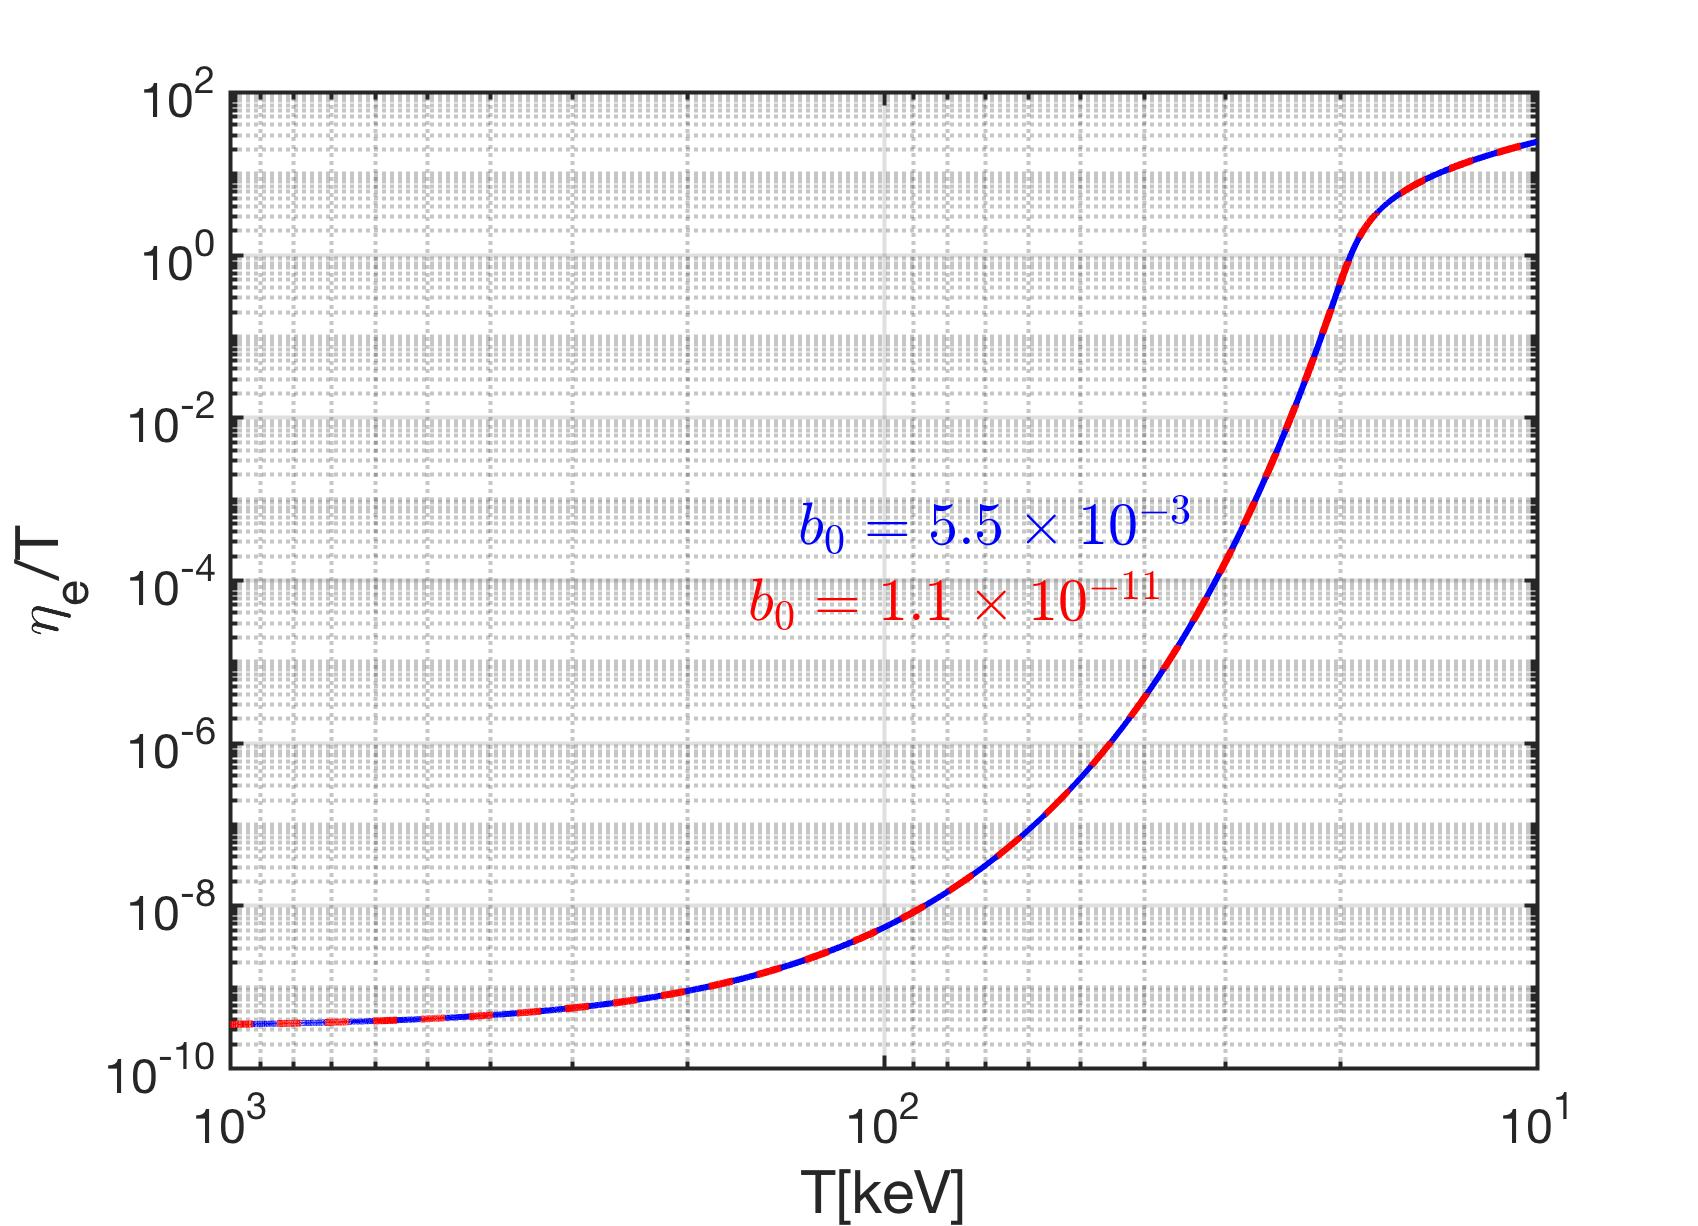
\includegraphics[width=\linewidth]{./plots/ChemicalPotential_new_survey}
\caption{The chemical potential of electron as a function of temperature in the magnetic field $b_0$ with $X_p=0.878$ and $n_B/n_\gamma=6.05\times10^{-10}$. The red dashed line represents the magnetic field $b_0=1.1\times10^{-11}$ and blue line labels the magnetic field $b_0=5.5\times10^{-3}$}
\label{ChemicalPotential_B}
\end{center}
\end{figure}
%~~~~~~~~~~~~~~~~~~~~~~~~~~~~~~~~~~~~~~~~

\subsubsection{Electron-positron magnetization}
%We consider the electron-positron plasma in the mean field approximation where the external field is representative of the \lq\lq bulk\rq\rq\ internal magnetization of the gas. Each particle is therefore responding to the averaged magnetic flux generated by its neighbors as well as any global external field contribution. 

Considering the magnetized electron-positron partition function Eq.~(\ref{lnZ}), it is convenient to introduce the dimensionless magnetization $\overline{\mathcal{M}}$ and the critical field $B_c$ as follows
\begin{align}
\label{Mdef}
\overline{\mathcal{M}}\equiv\frac{M}{\mathcal{B}_{c}}=\frac{1}{\mathcal{B}_{c}}\left(\frac{T}{V}\frac{\partial \ln\mathcal{Z}_{tot}}{\partial B}\right)\,\qquad \mathcal{B}_{c}=\frac{m_{e}^{2}}{e}\,.
\end{align}
Substituting the partition function Eq.~(\ref{lnZ}) into Eq.~(\ref{Mdef}), the total magnetization ${\overline{\mathcal M}}$ can be broken into the sum of spin parallel $\overline{\mathcal M}_{+}$ and spin anti-parallel $\overline{\mathcal M}_{-}$ magnetization. We have
\begin{align}\label{Magnetization}
&{\overline{\mathcal M}}={\overline{\mathcal M}_+}+{\overline{\mathcal M}_-},\\
&\overline{\mathcal M}_{\pm}=\frac{e^2T^{2}}{2\pi^2m_e^2}\left[2\cosh\left(\frac{\eta_{e}}{T}\right)\right]\left\{c_{1}(x_{\pm})K_1(x_i)+c_{0}K_0(x_\pm)\right\}\,,
\end{align}
where the coefficients are given by
\begin{align}
    c_{1}(x_{\pm}) &= \left[\frac{1}{2}-\left(\frac{1}{2}\pm\frac{g}{4}\right)\left(1+\frac{b^2_0}{12x^2_\pm}\right)\right]x_\pm\,,\qquad c_{0} = \left[\frac{1}{6}-\left(\frac{1}{4}\pm\frac{g}{8}\right)\right]b_0\,.
\end{align}
Substituting the chemical potential Eq.~(\ref{ChemicalPotential}) into Eq.~(\ref{Magnetization}), we can solve the magnetization numerically.
%~Figure~~~~~~~~~~~~~~~~~~~~~~~~~~~~~
\begin{figure}[ht]
    \centering
    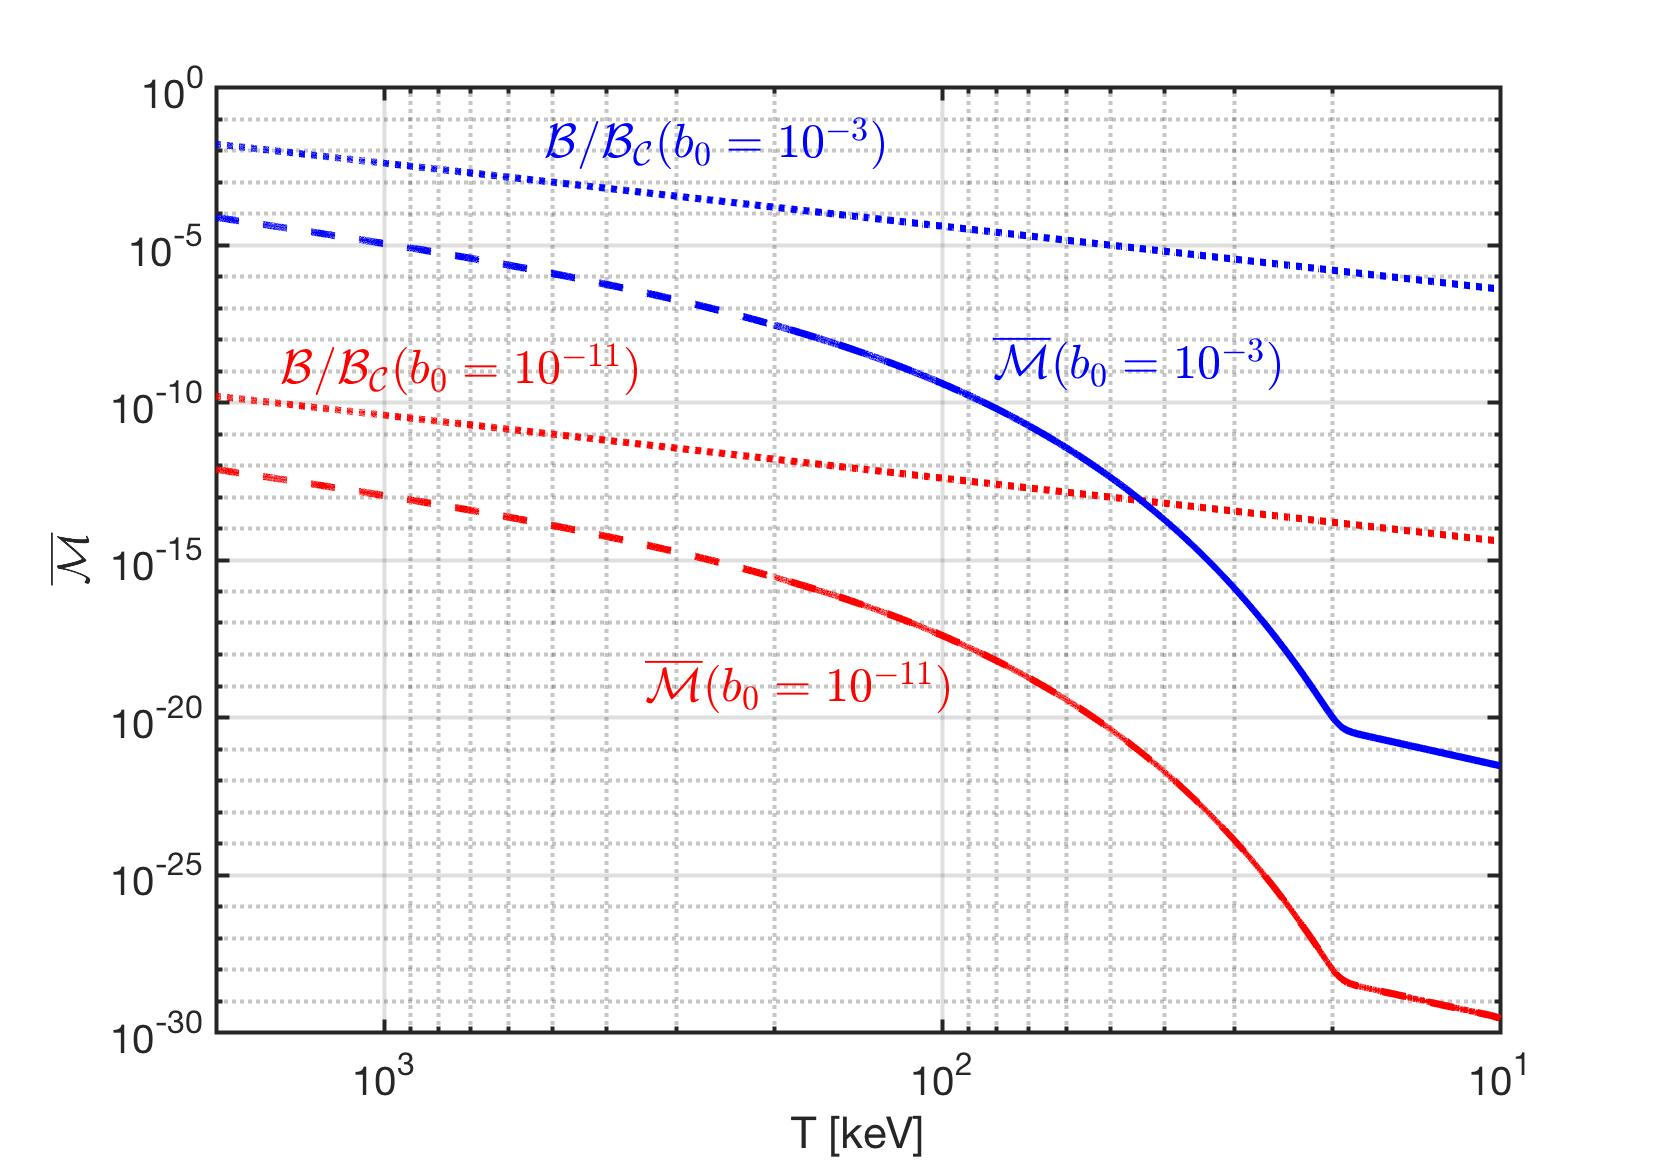
\includegraphics[width=\textwidth]{./plots/Magnetization_Hc_new002.jpg}
    \caption{The magnetization $\overline{\cal M}=\mathcal{M}/\mathcal{B}_C$, with $g=2$, of the primordial $e^{+}e^{-}$ plasma is plotted as a function of temperature. The lower (solid red) and upper (solid blue) bounds for cosmic magnetic scale $b_{0}$ are included. The external magnetic field strength ${\cal B}/{\cal B}_{C}$ is also plotted in for lower (dashed red) and upper (dashed blue) bounds. The spin fugacity is set to unity.}
    \label{fig:magnet} 
\end{figure}
%~Figure~~~~~~~~~~~~~~~~~~~~~~~~~~~~~

In this thesis we focus on considering the case for $g=2$. In this case, the electron-positron magnetization can be written as 
\begin{align}\label{Magnetization_g2}
&{\overline{\mathcal M}}={\overline{\mathcal M}_+}+{\overline{\mathcal M}_-}\\
&{\overline{\cal M}}_{+}=\frac{e^{2}}{\pi^{2}}\frac{T^{2}}{m_{e}^{2}}\cosh{\frac{\eta_e}{T}}\left[\frac{1}{2}x_{+}K_{1}(x_{+})+\frac{b_{0}}{6}K_{0}(x_{+})\right]\,,\\
&{\overline{\cal M}}_{-}=-\frac{e^{2}}{\pi^{2}}\frac{T^{2}}{m_{e}^{2}}\cosh{\frac{\eta_e}{T}}\left[\left(\frac{1}{2}+\frac{b_{0}^{2}}{12x_{-}^{2}}\right)x_{-}K_{1}(x_{-})+\frac{b_{0}}{3}K_{0}(x_{-})\right]\,,
\end{align}
where $x_\pm$ are given by
\begin{align}
x_{+}=\frac{m_{e}}{T},\qquad   x_{-}=\sqrt{\frac{m_{e}^{2}}{T^{2}}+2b_{0}}
\end{align}
The discussion for the case $g\neq2$ can be found in~~[\cite{Andrew:2023abc}].

In Fig.~\ref{fig:magnet}, we present the magnetization Eq.~(\ref{Magnetization_g2}) for the case $g=2$ as a function of temperature. It shows that the magnetization depends on the magnetic scale $b_0$ and the $e^{+}e^{-}$ plasma possesses an overall paramagnetic property, resulting in a positive magnetization $\overline{\mathcal{M}}$. This paramagnetic property is contrary to the conventional assumption that matter-antimatter plasmas lack significant inherent magnetic responses. However, the magnetization never exceeds the external field under the parameters considered, which shows a lack of ferromagnetic behavior. As the Universe cooled, the dropping magnetization slowed at $T_{\mathrm{split}}=20.3$ keV, where positrons vanished. Thereafter the remaining electron density diluted with cosmic expansion.

In this section, we have explored the electron-positron plasma considering  external and self-magnetization fields  without spin potential $\eta_s/T\ll1$. However the nonzero spin potential $\eta_s\neq0$  would have an impact on the primordial $e^{+}e^{-}$ plasma. In general, the  magnetization is also a function of the spin potential $\eta_s$, and would be one important parameter that control the spin direction of primordial gas which allows for magnetization even in the absence of external magnetic fields. For further discussion see ~[\cite{Andrew:2023abc}].



